\documentclass[conference]{IEEEtran}

\IEEEoverridecommandlockouts

% ---------------------------------------------------------------- packages
\usepackage{cite}
\usepackage{amsmath,amssymb}
\usepackage{graphicx}
\usepackage{booktabs}
\usepackage{array}
\usepackage{multirow}
\usepackage{tabularx}
\usepackage{adjustbox}
\usepackage{xcolor}
\usepackage{algorithm}
\usepackage{algpseudocode}
\usepackage{listings}
\usepackage{tikz}
\usetikzlibrary{shapes.geometric,arrows.meta,positioning,fit,calc,backgrounds}
\usepackage{textcomp}
\usepackage[hidelinks]{hyperref}

\newcommand{\code}[1]{\texttt{#1}}
\providecommand{\textasciicircum}{\^{}}

% --------------------------------------------------------------- listings
\definecolor{codegreen}{rgb}{0,0.5,0}
\lstdefinelanguage{MedScript}{
    morekeywords={input,const,func,let,if,else,while,return,true,false,int,float,bool,string,phi,range},
    morekeywords=[2]{kg,lb,gram,mg,ml,bpm,mmHg,degC,degF,metre,hour},
    morekeywords=[3]{print,export,present,anonymize,lb_to_kg,degF_to_degC,g_to_mg,abs,min,max},
    keywordstyle=\color{blue}\bfseries,
    keywordstyle=[2]\color{orange!80!black},
    keywordstyle=[3]\color{purple},
    sensitive=true, morecomment=[l]{//}, morestring=[b]"
}
\lstset{
    language=C, basicstyle=\ttfamily\fontsize{6.5}{7.5}\selectfont,
    keywordstyle=\color{blue}, commentstyle=\color{codegreen}, stringstyle=\color{violet},
    numbers=none, frame=single, breaklines=true, breakindent=0pt, showstringspaces=false,
    xleftmargin=0.2em, xrightmargin=0.2em, columns=fullflexible, aboveskip=4pt, belowskip=2pt
}

\newcommand{\NProg}{10{,}000}
\newcommand{\NFeat}{101}
\newcommand{\NTrain}{8{,}000}
\newcommand{\NTest}{2{,}000}
\newcommand{\MeanLoc}{38.7}
\newcommand{\TotalLoc}{386{,}953}
\newcommand{\NDouble}{1{,}398}
\newcommand{\DoubleShare}{15.5}
\newcommand{\RuleFirstAcc}{91.6}
\newcommand{\RulePrioAcc}{93.2}
\newcommand{\RuleFirstDouble}{65.7}
\newcommand{\RFAcc}{99.15}
\newcommand{\MLPAcc}{99.35}
\newcommand{\HGBAcc}{99.40}
\newcommand{\LRAcc}{99.20}
\newcommand{\RFMacro}{0.9915}
\newcommand{\RFDouble}{96.4}
\newcommand{\RuleLogicRecall}{68.5}
\newcommand{\RFLogicRecall}{97.0}
\newcommand{\MsPerKloc}{162}
\newcommand{\ScaleRSq}{0.981}
\newcommand{\ScaleSlope}{1.17}
\newcommand{\OptMean}{8.9}
\newcommand{\OptMax}{17.8}
\newcommand{\OptPrograms}{300}
\newcommand{\OptMismatch}{0}
\newcommand{\AugMinutes}{34}
\newcommand{\HeldoutNN}{7.4}


\begin{document}

\title{Intelligent Compiler for Detecting Errors in\\
Medical Data Processing Programs Using GAN\thanks{Course project for Compiler Design Lab (CSE3024), School of Computer
Science and Engineering (SCOPE), VIT-AP University. Compiler design component: parsing and semantic analysis.
Machine learning component: error classification. Application domain: healthcare.}}

\author{\IEEEauthorblockN{Swarnim Bandekar}
\IEEEauthorblockA{\textit{School of Computer Science and Engineering (SCOPE)}\\
\textit{VIT-AP University}\\
Amaravati, Andhra Pradesh, India\\
Regd. No. 24BCB7157}
\and
\IEEEauthorblockN{Lithin CG}
\IEEEauthorblockA{\textit{School of Computer Science and Engineering (SCOPE)}\\
\textit{VIT-AP University}\\
Amaravati, Andhra Pradesh, India\\
Regd. No. 24BCB7016}}

\maketitle

\begin{abstract}
Programs that process medical data can contain mistakes that a general-purpose compiler never reports: a dose added to a
body weight, a temperature threshold typed ten times too large, a laboratory value that may be missing but is used
unguarded, or a patient name that reaches a log file. This paper describes a compiler front end built to catch such
errors, and a learned classifier that names the root-cause family of each defective program. The front end is written for
MedScript, a small domain-specific language with units of measure in its types, declared physiological ranges,
protected-health-information tagging and optional values. It comprises a hand-written lexer, a recursive-descent parser with
error recovery, and a semantic analyser that checks types, units, range plausibility, taint flow of patient identifiers,
optional values, definite assignment and division by zero; a three-address-code generator and optimiser complete the
pipeline. On a synthetic corpus of \NProg{} programs in ten classes, classifiers using compiler-derived features reach
\RFAcc\% accuracy, against \RuleFirstAcc\% for the family of the first diagnostic, and they catch faults the compiler cannot see,
such as an inverted fever rule. A conditional generative adversarial network (GAN) trained to augment rare error classes did not
help: Gaussian jitter and SMOTE performed better, and only about 4\% of the GAN's samples were recognisable as the requested class.
A GAN discriminator trained on valid programs did detect the compiler-invisible faults well (AUROC 0.98). The corpus is synthetic,
and the results should be read accordingly.
\end{abstract}

\begin{IEEEkeywords}
compiler design, semantic analysis, parsing, units of measure, error classification, generative adversarial network,
healthcare software
\end{IEEEkeywords}

% ============================================================
% INTRODUCTION
% ============================================================
\section{Introduction}\label{sec:intro}

Programs that handle medical data sit in an unusual place in the software landscape.
They are usually small and unglamorous---a script that flags abnormal vital signs, a routine that converts a
body weight into a drug dose, a nightly job that exports records to a research registry---yet a mistake in any
of them can reach a patient. Two accidents are often quoted to show how little it takes. The Therac-25 radiation
overdoses of the mid-1980s were traced to defects in control software \cite{leveson1993}, and the Mars Climate
Orbiter was lost in 1999 because one team produced impulse data in pound-force seconds while the consuming
software expected newton seconds \cite{mco1999}. The second failure is, in compiler terms, a plain type error
that the type system of the day simply could not see: both quantities were just \code{double}.

Clinical code has the same weak spot. A dose in milligrams added to a weight in kilograms, a temperature
threshold typed as \code{380} instead of \code{38.0}, a blood-glucose reading that may be missing from the
laboratory feed but is used as if it were always present, or a patient name that reaches a log file without
being anonymised: each of these is syntactically fine and passes through a general-purpose compiler without a
word. The relevant knowledge---units, physiological ranges, privacy rules---lives in the heads of the people who
write the program, not in the language they write it in.

This project builds a small compiler front end that \emph{does} know about that domain, and then asks a
machine-learning question on top of it: once a program has been rejected (or, worse, accepted), can a learned
model tell us what kind of mistake it contains, even when the compiler's own diagnostics are incomplete or
misleading? The generative adversarial network (GAN) enters the picture for a practical reason. Labelled
examples of faulty medical programs are scarce, and they are awkward to share because real clinical scripts tend
to embed identifiers and institutional rules. A conditional GAN that learns the distribution of compiler-derived
feature vectors per error class offers a way to produce additional training records without handing over any
source code. Whether that actually helps is an empirical question, and we report the answer as we measured it,
including the places where it did not help.

\subsection{Motivation}

Three observations motivated the work.

\begin{enumerate}
    \item \textbf{General compilers are blind to domain constraints.} Mainstream languages check that an
    expression is a number, not that it is a mass. Units-of-measure systems exist
    \cite{kennedy1994} but are not part of the languages most clinical scripting is done in.
    \item \textbf{Rule-based diagnostics are precise but narrow.} A hand-written analyser reports exactly what it
    was told to look for. It says nothing about an inverted fever rule such as
    \code{if (temp < 38.0 degC)} followed by an alert called ``fever'', because nothing in the grammar or the
    type system is violated. Cascading faults make things worse: when several defects coexist, the first message
    is not necessarily the root cause.
    \item \textbf{Labelled data is the bottleneck.} Learning-based bug finders depend on large corpora
    \cite{allamanis2018,pradel2018}. In a regulated domain the corpus of real faulty programs is small, and
    synthetic augmentation is attractive if it can be shown to work.
\end{enumerate}

The course context also shaped the design. The assignment asks for a compiler component---here parsing and
semantic analysis---and a machine-learning component---here error classification---applied to a concrete
domain, which for us is healthcare. We therefore treated the compiler as the primary artefact and the learned
model as a second stage that consumes what the compiler produces.

\subsection{Problem Statement}

The problem addressed in this paper is:

\begin{quote}
\textit{Given the source text of a medical data-processing program, how can we (i) detect domain-specific
errors---unit, range, privacy and missing-value errors in addition to ordinary lexical, syntactic and type
errors---with a purpose-built compiler front end, and (ii) assign each defective program to its root-cause error
family with a learned classifier that is trained on compiler-derived features, using a generative adversarial
network to compensate for the scarcity of labelled faulty programs?}
\end{quote}

\subsection{Objectives}

\begin{enumerate}
    \item To design \emph{MedScript}, a small imperative language for medical data processing with first-class
    units of measure, protected-health-information (PHI) tagging, optional (possibly missing) values and
    declared physiological ranges.
    \item To implement a complete front end for it: a hand-written lexer, a recursive-descent parser with error
    recovery, and a semantic analyser that performs type, unit, range, taint, missing-value, definite-assignment
    and division-by-zero checks.
    \item To implement the back end far enough to demonstrate the compiler pipeline end to end: three-address
    code, constant folding, constant propagation, common-subexpression elimination, dead-code elimination, and a
    reference virtual machine used to check that optimisation preserves behaviour.
    \item To define a taxonomy of ten classes (valid plus nine error families), build a labelled corpus of valid and fault-injected
    programs, and train classifiers on features extracted from the compiler's tokens, syntax tree and
    diagnostics.
    \item To train conditional GANs on those features and measure honestly whether the synthetic records improve
    classification when real faulty examples are scarce, and whether a GAN trained only on valid programs can
    serve as an anomaly detector.
    \item To measure the compiler itself: scaling of compilation time with program size and the effect of
    optimisation on code size.
\end{enumerate}

\subsection{Contributions}

The main contributions of this paper are:

\begin{itemize}
    \item \textbf{MedScript and its compiler.} A domain-specific language and a Python implementation (about
    1{,}900 lines for the compiler proper, about 4{,}900 including corpus tools, learning code, experiments and tests)
    of lexer, parser, semantic analyser, IR generator, optimiser and virtual machine, with a command-line tool that also reports a learned root-cause estimate. A suite of 38 unit tests accompanies it.
    \item \textbf{Semantic analysis that encodes clinical safety rules.} Unit checking through exponent vectors
    over base units, interval reasoning over declared ranges, taint tracking from \code{phi} inputs to output
    sinks, and flow-sensitive refinement of optional values.
    \item \textbf{A fault-injection corpus.} \NProg{} programs in ten classes, produced by 46 mutation operators
    with a check that each injected fault actually manifests, including \DoubleShare\% multi-fault programs among
    the faulty ones.
    \item \textbf{A comparison of rule-based and learned error classification.} The learned classifiers reach
    \RFAcc\% accuracy against \RuleFirstAcc\% for the ``first diagnostic'' rule, and they also catch faults the
    compiler cannot see, which neither rule baseline does.
    \item \textbf{An honest evaluation of GAN augmentation.} Seven training regimes are compared over ten
    random seeds at five levels of data scarcity, together with fidelity measurements of the synthetic records
    and a GAN-based anomaly detector. The GAN turns out not to help, and the paper says why.
\end{itemize}

\subsection{Organisation of the Paper}

Section~\ref{sec:related} reviews related work. Section~\ref{sec:method} describes the language, the compiler phases and the machine-learning
components. Section~\ref{sec:setup} describes the corpus, the experimental protocol and the software environment. Section~\ref{sec:results}
presents and discusses results. Section~\ref{sec:concl} concludes and outlines future work. The appendices contain the full
grammar, the diagnostic catalogue, the fault operators and a short guide to running the code.


% ============================================================
% RELATED WORK
% ============================================================
\section{Related Work}\label{sec:related}

The project touches four bodies of work: classical compiler front ends, static analyses for domain-specific
properties such as units and information flow, machine learning for program defects, and generative models and
resampling for imbalanced data. This section summarises each and then states where our work sits.

\subsection{Classical Compiler Front Ends}

The standard treatment of lexical analysis, parsing and semantic analysis is that of Aho et
al.~\cite{aho2006}; Cooper and Torczon~\cite{cooper2007} and Appel~\cite{appel1998} cover the same ground with
more attention to implementation. Two ideas from that literature are used directly in this project. The first is
\emph{error recovery}. A compiler that stops at the first syntax error is unpleasant to use, so parsers
resynchronise: they either skip tokens until a safe point (panic mode) or repair the input locally by inserting
or deleting a token. Burke and Fisher~\cite{burke1987} give a systematic method for LR and LL parsers, and Grune
and Jacobs~\cite{grune2008} survey the alternatives. Our recursive-descent parser combines both: a missing
semicolon or parenthesis is reported and treated as if it had been present, and any other malformed construct is
skipped up to the next statement boundary. The second idea is \emph{phase gating}: later phases are only run on
an input that earlier phases accepted, because a semantic analysis of a tree built from broken syntax produces
noise. We follow this convention, which, as Section~\ref{sec:results} shows, has a measurable effect on what the compiler can
tell about programs that contain several faults.

Type checking itself is covered by Pierce~\cite{pierce2002}. The flow-sensitive parts of our semantic
analyser---definite assignment, and the refinement of optional values inside a guarded branch---are instances of
the data-flow framework presented by Nielson et al.~\cite{nielson1999}.

\subsection{Units of Measure and Information-Flow Analysis}

Kennedy's \emph{dimension types}~\cite{kennedy1994} extend a type system so that numeric types carry a unit
expressed as a product of base units raised to integer powers. Multiplication adds exponents, division subtracts
them, and addition requires equal exponents. This is precisely the rule that would have caught the Mars Climate
Orbiter error and the dose-plus-weight mistake mentioned in the introduction, and it is the formulation used here.

Taint analysis tracks data from \emph{sources} to \emph{sinks}. TaintDroid~\cite{enck2010} applies it dynamically
to detect private data leaving a smartphone. We use a simple static variant: values read from inputs marked
\code{phi} are tainted, taint propagates through arithmetic, string concatenation and user functions, and it is
cleared only by an explicit \code{anonymize()} call. Reaching \code{print} or \code{export} with a tainted value is
an error. The motivation is regulatory rather than technical: the HIPAA Privacy Rule restricts the disclosure of
individually identifiable health information and describes de-identification procedures~\cite{hipaa}.

\subsection{Machine Learning for Program Defects}

Allamanis et al.~\cite{allamanis2018} survey the use of statistical models of source code, building on the
observation that real programs are repetitive and predictable~\cite{hindle2012}. DeepFix~\cite{gupta2017} trains a
sequence-to-sequence network to repair common syntax and type errors in student C programs. DeepBugs~\cite{pradel2018}
learns from name-based features to flag bugs such as swapped arguments and wrong binary operators---close in
spirit to the inverted-comparison faults we study. Graph neural networks over syntax and data-flow edges have
also been used to detect variable misuse~\cite{allamanis2018graphs}. These systems work on general-purpose code and
operate on tokens or graphs. We take a different, lighter route: the learned model sees \emph{what the compiler
already computed}---counts of each diagnostic, structural statistics, and a few clinical-rule patterns---which
keeps the model small, makes its inputs inspectable, and lets it use the compiler as a feature extractor rather than
re-learning grammar.

\subsection{GANs, Augmentation and Imbalanced Learning}

A generative adversarial network trains a generator $G$ and a discriminator $D$ in a two-player game
\cite{goodfellow2014}; the conditional variant feeds a class label to both networks so that samples can be drawn for a
chosen class~\cite{mirza2014}. Training can be unstable, and a large part of the subsequent literature addresses
that: label smoothing and related heuristics~\cite{salimans2016}, the Wasserstein objective~\cite{arjovsky2017} and
its gradient-penalty form~\cite{gulrajani2017}. In healthcare, medGAN~\cite{choi2017} generates synthetic patient
records, and CTGAN~\cite{xu2019} handles mixed tabular data; the Data Augmentation GAN~\cite{antoniou2017} was
proposed specifically for the low-data regime. For class imbalance, the classical alternatives are random
oversampling and SMOTE~\cite{chawla2002}, which interpolates between a minority sample and one of its nearest
neighbours; He and Garcia~\cite{he2009} review the field. A GAN can also serve as an anomaly detector: AnoGAN
\cite{schlegl2017} trains on normal data only and scores an input by how poorly the generator can reproduce it. We use
a lighter-weight version of this idea, scoring with the discriminator or critic, and compare it with Isolation
Forest~\cite{liu2008} and the one-class SVM~\cite{scholkopf2001}.

\subsection{Survey of Related Approaches}

\begin{table*}[t]
\centering
\caption{Related approaches compared with the system built in this project.}
\label{tab:survey}
\footnotesize
\begin{tabularx}{\textwidth}{p{2.6cm}p{2.5cm}Xp{3.0cm}}
\toprule
\textbf{Approach} & \textbf{Domain} & \textbf{Main idea} & \textbf{Limitation for our setting}\\
\midrule
Classical front end \cite{aho2006} & General languages & Lexing, parsing, type checking & Blind to units, ranges, PHI\\
Dimension types \cite{kennedy1994} & Scientific code & Units as exponent vectors & No privacy or missing-value rules\\
TaintDroid \cite{enck2010} & Mobile apps & Dynamic information-flow tracking & Runtime only; no clinical semantics\\
DeepFix \cite{gupta2017} & Student C programs & Seq2seq repair of syntax/type errors & Needs large labelled corpus\\
DeepBugs \cite{pradel2018} & JavaScript & Name-based bug classifiers & No domain knowledge\\
SMOTE \cite{chawla2002} & Tabular data & Interpolate minority neighbours & Not generative; stays inside the convex hull\\
medGAN / CTGAN \cite{choi2017,xu2019} & Patient records / tables & GAN-based synthetic records & Not applied to program features\\
AnoGAN \cite{schlegl2017} & Medical images & Anomaly scoring with a GAN & Images, not programs\\
\textbf{This work} & Medical-data programs & Domain-aware front end $+$ learned error-family classifier with GAN augmentation & Synthetic corpus; DSL rather than a mainstream language\\
\bottomrule
\end{tabularx}
\end{table*}

\subsection{Gap and Positioning}

None of the surveyed systems combines (a) a front end with built-in clinical semantics, (b) a learned classifier that
sits on top of that front end and reasons about root cause, and (c) an explicit evaluation of GAN-based augmentation
against simple resampling baselines in the same setting. That combination is what this project attempts. It does so at
laboratory scale: the language is a purpose-built DSL, and the corpus is synthetic. We return to the consequences of
those choices in Section~\ref{sec:threats}.

\subsection{Limitations of Existing Approaches}

Several limitations of existing approaches shaped our design choices:

\begin{enumerate}
    \item General-purpose compilers do not check units, ranges, privacy or missingness, so the most dangerous
    clinical mistakes pass silently.
    \item Rule-based analyses are precise but incomplete; they cannot flag a rule that is merely \emph{wrong}.
    \item With several coexisting faults, the first reported diagnostic may not be the root cause, and phase gating hides
    later-phase faults entirely.
    \item Learned bug detectors require large corpora, which regulated domains cannot provide.
    \item GAN training is unstable and data-hungry, and its benefit over cheap resampling is rarely tested on the same
    task.
\end{enumerate}


% ============================================================
% PROPOSED METHODOLOGY
% ============================================================
\section{Proposed Methodology}\label{sec:method}

\subsection{System Overview}

The system has two cooperating halves, shown in Fig.~\ref{fig:arch}. The \emph{compiler half} is a conventional
pipeline---scanner, parser, semantic analyser, intermediate-code generator, optimiser---for a domain-specific
language called MedScript. Every phase reports diagnostics with a stable code, a position and a message. The
\emph{learning half} takes what the compiler produced (tokens, syntax tree, diagnostics) and condenses it into a
fixed-length feature vector. A classifier maps that vector to one of ten classes: \emph{valid} or one of nine error
families. A conditional GAN, trained on feature vectors of the labelled corpus, supplies extra synthetic records of
the rare classes at training time. At inference time the GAN is not used; the deployed artefact is the compiler plus
a random-forest classifier.

\begin{figure*}[t]
\centering
\resizebox{\textwidth}{!}{%
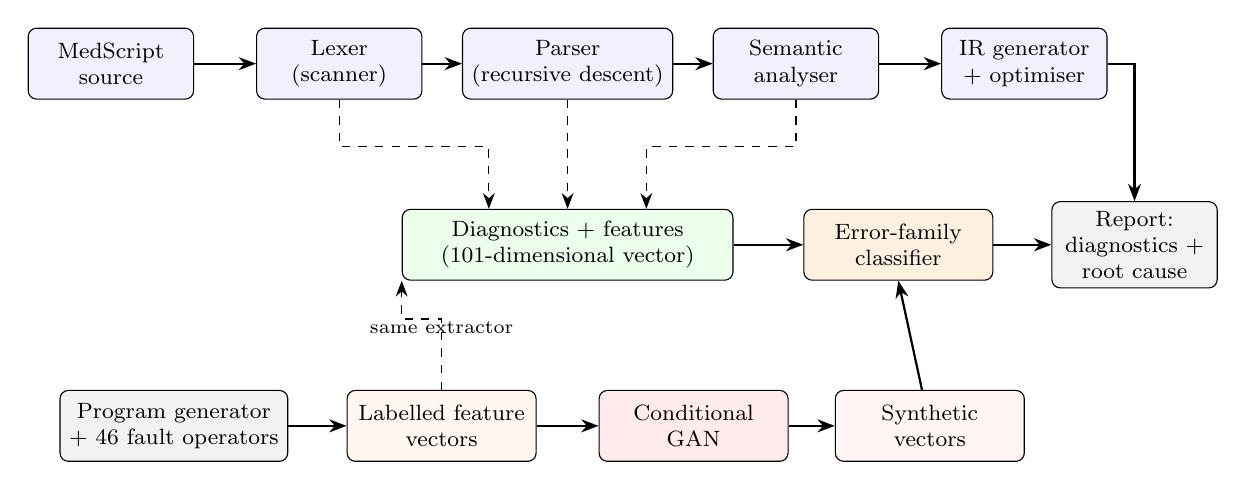
\begin{tikzpicture}[
  box/.style={rectangle,rounded corners=3pt,draw,minimum height=0.9cm,minimum width=2.1cm,align=center,font=\footnotesize,fill=blue!6},
  ml/.style={rectangle,rounded corners=3pt,draw,minimum height=0.9cm,minimum width=2.4cm,align=center,font=\footnotesize,fill=orange!12},
  gan/.style={rectangle,rounded corners=3pt,draw,minimum height=0.9cm,minimum width=2.4cm,align=center,font=\footnotesize,fill=red!8},
  arr/.style={-{Stealth[length=2.2mm]},thick},
  dsh/.style={-{Stealth[length=2mm]},dashed}
]
\node[box] (src) at (0,0) {MedScript\\source};
\node[box] (lex) at (2.9,0) {Lexer\\(scanner)};
\node[box] (par) at (5.8,0) {Parser\\(recursive descent)};
\node[box] (sem) at (8.7,0) {Semantic\\analyser};
\node[box] (ir)  at (11.6,0) {IR generator\\+ optimiser};
\draw[arr] (src) -- (lex);
\draw[arr] (lex) -- (par);
\draw[arr] (par) -- (sem);
\draw[arr] (sem) -- (ir);

\node[box,fill=green!8,minimum width=4.2cm] (diag) at (5.8,-2.3) {Diagnostics + features\\(101-dimensional vector)};
\draw[dsh] (lex.south) -- ++(0,-0.6) -| ($(diag.north)+(-1.0,0)$);
\draw[dsh] (par.south) -- (diag.north);
\draw[dsh] (sem.south) -- ++(0,-0.6) -| ($(diag.north)+(1.0,0)$);

\node[ml] (clf) at (10.0,-2.3) {Error-family\\classifier};
\draw[arr] (diag) -- (clf);
\node[box,fill=gray!10] (rep) at (13.0,-2.3) {Report:\\diagnostics +\\root cause};
\draw[arr] (clf) -- (rep);
\draw[arr] (ir) -- (13.0,0) -- (rep.north);

\node[box,fill=gray!10] (gen) at (0.8,-4.6) {Program generator\\+ 46 fault operators};
\node[ml,fill=orange!6] (corp) at (4.2,-4.6) {Labelled feature\\vectors};
\node[gan] (cg) at (7.4,-4.6) {Conditional\\GAN};
\node[gan,fill=red!4] (syn) at (10.4,-4.6) {Synthetic\\vectors};
\draw[arr] (gen) -- (corp);
\draw[arr] (corp) -- (cg);
\draw[arr] (cg) -- (syn);
\draw[arr] (syn) -- (clf.south);
\draw[dsh] (corp.north) -- ++(0,0.9) -| (diag.south west);
\node[font=\scriptsize,align=center] at (4.2,-3.35) {same extractor};
\end{tikzpicture}}
\caption{Architecture of the proposed system. Solid arrows are data flow, dashed arrows are diagnostics and features
collected from the compiler phases. The GAN branch (bottom) is used only to enlarge the training set.}
\label{fig:arch}
\end{figure*}

\subsection{The MedScript Language}

MedScript is deliberately small: it contains just enough to express the programs a clinical-informatics student
might write, and just enough machinery to make the domain-specific checks meaningful. Its main design decisions
are the following.

\begin{itemize}
    \item \textbf{Units are part of the type.} A numeric type is \code{int}, \code{float}, or a float tagged with a
    unit expression such as \code{kg}, \code{mg/kg} or \code{kg/metre\textasciicircum 2}. Literals carry units:
    \code{38.0 degC}, \code{15 mg/kg}.
    \item \textbf{Inputs are declared with metadata.} \code{input weight: kg range(2, 300);} declares a read-only
    patient quantity with a physiological range. \code{phi} marks protected health information.
    \item \textbf{Optional values.} A trailing \code{?} (as in \code{mg/ml?}) means the value may be missing. It
    must be tested with \code{present(x)} before use.
    \item \textbf{Two output sinks.} \code{print} and \code{export}; both reject PHI unless it passed through
    \code{anonymize}.
    \item \textbf{Ordinary control flow.} \code{if}/\code{else}, \code{while}, functions with typed parameters and
    return types, \code{let} bindings with optional type inference.
\end{itemize}

Table~\ref{tab:units} lists the unit vocabulary. The single-letter units one might expect (\code{m}, \code{g},
\code{h}) are spelled \code{metre}, \code{gram} and \code{hour}, so that those short names stay available as
identifiers.

\begin{table}[t]
\centering
\caption{Units of measure known to the compiler and the plausibility bounds used for literals.}
\label{tab:units}
\footnotesize
\begin{tabular}{llr}
\toprule
\textbf{Unit} & \textbf{Meaning} & \textbf{Plausible literal range}\\
\midrule
\code{kg}, \code{lb} & body mass & 0.2--500 kg;\ 0.4--1100 lb\\
\code{gram}, \code{mg} & mass of substance & 0--20 g;\ 0--20000 mg\\
\code{ml}, \code{hour} & volume, time & 0--10000 ml;\ 0--72 h\\
\code{bpm} & beats (or breaths) per minute & 0--300\\
\code{mmHg} & blood pressure & 0--350\\
\code{degC}, \code{degF} & temperature & 20--45 $^\circ$C;\ 68--113 $^\circ$F\\
\code{metre} & body height & 0.2--2.5\\
\bottomrule
\end{tabular}
\end{table}

A complete program that the compiler accepts is shown in Listing~\ref{lst:ok}. It computes a weight-based dose with
a safety cap, a body-mass index, a fever alert, a sepsis screen, an alert that is guarded for a possibly missing
laboratory value, and an anonymised export.

\begin{lstlisting}[language=MedScript,caption={A valid MedScript program (\texttt{examples/triage\_ok.med}).},label={lst:ok}]
input patient_name: string phi;
input weight: kg range(2, 300);
input height: metre range(0.4, 2.3);
input temp: degC range(30, 43);
input hr: bpm range(20, 250);
input lactate: mg? range(0, 400);

const MAX_DOSE: mg = 1000 mg;

func dose_for(w: kg, rate: mg/kg) -> mg {
    let d: mg = rate * w;
    if (d > MAX_DOSE) { return MAX_DOSE; }
    return d;
}
func bmi(w: kg, h: metre) -> kg/metre^2 {
    return w / (h * h);
}

let dose: mg = dose_for(weight, 15 mg/kg);
let index = bmi(weight, height);
let fever = false;
if (temp > 38.0 degC) { fever = true; print("fever alert"); }
if (hr > 100 bpm && fever) { print("sepsis screen"); }
if (present(lactate)) {
    if (lactate > 200 mg) { print("high lactate"); }
}
export(anonymize(patient_name));
print(dose);
print(index);
\end{lstlisting}

\subsection{Lexical Analysis}

The scanner is a hand-written, single-pass, longest-match recogniser. The token classes are summarised in
Table~\ref{tab:tokens}. Identifiers and keywords share one regular expression; the lexeme is then looked up in the
keyword set and in the unit set. A numeric lexeme is first collected as the maximal run of letters, digits and dots
and \emph{then} validated against $[0\text{-}9]^+(.[0\text{-}9]^+)?$; this way \code{3.4.5} and \code{10x} are reported as one
malformed number rather than as a number followed by stray characters.

\begin{table}[t]
\centering
\caption{Token classes of MedScript.}
\label{tab:tokens}
\footnotesize
\begin{tabular}{p{1.1cm}p{4.2cm}p{2.5cm}}
\toprule
\textbf{Class} & \textbf{Pattern} & \textbf{Examples}\\
\midrule
\code{ID} & letter or underscore, then letters, digits, underscores (minus keywords and units) & \code{weight}, \code{dose\_for}\\
Keyword & fixed set of 16 words & \code{input}, \code{if}, \code{phi}, \code{range}\\
\code{UNIT} & fixed set of 11 words & \code{kg}, \code{mmHg}, \code{degC}\\
\code{NUM} & digits, optionally a dot and more digits & \code{38}, \code{0.45}\\
\code{STR} & double quote, any characters except quote and newline, double quote & \code{"ALERT fever"}\\
Operators & \code{+ - * / \% < > <= >= == != \&\& || ! = ->} & \\
Punctuation & \code{( ) \{ \} , ; : ? \textasciicircum} & \\
Comment & \code{//} to end of line (discarded) & \\
\bottomrule
\end{tabular}
\end{table}

Three lexical diagnostics exist: an illegal character (\code{LEX001}), a malformed number (\code{LEX002}) and an
unterminated string (\code{LEX003}). Each is \emph{recoverable}: an illegal character is dropped, a malformed number
is replaced by its longest valid prefix, and an unterminated string consumes the rest of the line. The parser
therefore still receives a usable token stream, and later phases run normally. This detail matters for
classification: a lexical error does not hide semantic faults, whereas a syntax error does.

\subsection{Syntax Analysis}

The grammar (Appendix~\ref{app:grammar} gives it in full) is LL(1) apart from two decisions. When a statement begins with an
identifier, the parser must choose between an assignment and a call; it resolves this with one extra token of
lookahead (\code{ID =}). Likewise, after a number and a unit, a following \code{/} belongs to the unit expression
only if the token after it is also a unit. Expressions use precedence climbing over six levels, from \code{||}
(lowest) to the multiplicative operators. Table~\ref{tab:first} lists the tokens that can begin each kind of
statement, which are also the synchronisation points used for error recovery.

\begin{table}[t]
\centering
\caption{FIRST sets of the statement forms, used for prediction and as synchronisation tokens.}
\label{tab:first}
\footnotesize
\begin{tabular}{ll}
\toprule
\textbf{Construct} & \textbf{FIRST}\\
\midrule
input declaration & \code{input}\\
constant declaration & \code{const}\\
function declaration & \code{func}\\
let / if / while / return & \code{let}\ \ \code{if}\ \ \code{while}\ \ \code{return}\\
block & \code{\{}\\
assignment & \code{ID} followed by \code{=}\\
call statement / expression & \code{ID}, \code{NUM}, \code{STR}, \code{true}, \code{false}, \code{(}, \code{-}, \code{!}\\
\bottomrule
\end{tabular}
\end{table}

\paragraph{Error recovery.} Two mechanisms are combined. When a \emph{closing} token is missing---\code{;},
\code{)} or \code{\}}---the parser reports \code{SYN001}, anchors the message at the end of the previous token (where
a programmer would expect to see it), and carries on as if the token had been inserted. When an expression cannot
start (\code{SYN002}) the parser raises an internal resynchronisation exception that is caught at statement level;
the handler skips tokens until a semicolon is consumed or a token from Table~\ref{tab:first} is seen. At most one
diagnostic is issued per input position, which suppresses most duplicate cascades. A premature end of file yields
\code{SYN003}. If the parse produced \emph{any} syntax diagnostic, the semantic analyser is not run.

\subsection{Semantic Analysis}

The semantic analyser walks the tree once, keeping a stack of scopes and a small flow state. It is the part of the
compiler that carries the clinical knowledge, so we describe each check in turn.

\subsubsection{Symbol table and scopes}

Inputs and constants live in a global scope. Top-level \code{let} bindings live in a ``main'' scope layered above
it; function bodies see only the global scope, their parameters and their own locals. Functions are collected in a
first pass, so a call may precede the definition. Declaring a name twice in one scope is \code{SEM002}. A
\code{let} variable that is never read gives the warning \code{W002}.

\subsubsection{Types and units}

Let a numeric type be a pair $\tau[d]$ where $\tau\in\{\texttt{int},\texttt{float}\}$ and $d\in\mathbb{Z}^{U}$ is a
\emph{dimension vector}, one integer exponent per base unit $u\in U$. A plain number has $d=\mathbf{0}$; the type
\code{mg/kg} has exponent $+1$ for \code{mg}, $-1$ for \code{kg} and $0$ elsewhere. The typing rules for arithmetic are
\begin{align}
&\frac{\Gamma\vdash e_1:\tau_1[d_1]\quad\Gamma\vdash e_2:\tau_2[d_2]\quad d_1=d_2}
     {\Gamma\vdash e_1\pm e_2:\tau[d_1]}\\[4pt]
&\frac{\Gamma\vdash e_1:\tau_1[d_1]\quad\Gamma\vdash e_2:\tau_2[d_2]}
     {\Gamma\vdash e_1\cdot e_2:\tau[d_1+d_2]}\\[4pt]
&\frac{\Gamma\vdash e_1:\tau_1[d_1]\quad\Gamma\vdash e_2:\tau_2[d_2]}
     {\Gamma\vdash e_1/e_2:\texttt{float}[d_1-d_2]}
\end{align}
and comparison requires $d_1=d_2$ and yields \code{bool}. As an example, the product \code{rate * w} with
\code{rate}:\code{mg/kg} and \code{w}:\code{kg} has dimension $(+1)_{\text{mg}}+(-1)_{\text{kg}}+(+1)_{\text{kg}}=(+1)_{\text{mg}}$,
i.e., it is a mass in milligrams, which is exactly what the declaration \code{let d: mg = rate * w} expects.
Adding \code{weight + 5 lb} fails because $d_1\ne d_2$: \code{kg} and \code{lb} are distinct base units and the
language does not convert implicitly (conversion goes through \code{lb\_to\_kg}). The literal \code{0} is the only
dimension-polymorphic value, so that comparisons such as \code{x > 0} remain convenient.

A mismatch between base kinds (a string where a number is expected, a non-boolean condition, a wrong argument count)
is reported as \code{SEM004}, \code{SEM008} or \code{SEM006}; a mismatch of dimensions alone is \code{SEM005}. Keeping
the two apart is what lets the classifier distinguish the \emph{type} and \emph{unit} families later.

\subsubsection{Ranges and thresholds}

Every numeric value carries, besides its type, an optional closed interval $[l,h]$ obtained from the declared range
of an input or from interval arithmetic on constants:
\begin{align}
[a,b]+[c,d]&=[a+c,\,b+d],\\
[a,b]\cdot[c,d]&=[\min P,\max P],\quad P=\{ac,ad,bc,bd\},\\
[a,b]/[c,d]&=[a,b]\cdot[1/d,\,1/c],\quad\text{defined iff }0\notin[c,d].
\end{align}
Two checks use the intervals. (i) A literal that carries a single unit must lie inside the plausibility interval of
Table~\ref{tab:units}; \code{380 degC} does not. (ii) A comparison between an input with declared range $[l,h]$ and a
constant $k$ with $k<l$ or $k>h$ is flagged, because the comparison is then always true or always false. Both give
\code{DOM001}. A threshold exactly equal to a bound, such as \code{hr > 250 bpm} with \code{range(20, 250)}, is accepted.

\subsubsection{Division by zero}

A divisor whose constant value is $0$ gives \code{DOM004}. A divisor whose interval contains $0$ gives \code{DOM005},
unless a \emph{non-zero fact} is in force for that variable. Non-zero facts are produced by branch conditions such as
\code{x > 0}, \code{x != 0}, or the negation of \code{x <= 0}, and they hold inside the branch (or after an
early-returning branch that tests the opposite).

\subsubsection{PHI taint tracking}

Let $\mathrm{t}(e)\in\{0,1\}$ denote whether the value of expression $e$ may contain protected health information.
\begin{align}
\mathrm{t}(x)&=\mathit{phi}(x),\\
\mathrm{t}(e_1\odot e_2)&=\mathrm{t}(e_1)\lor\mathrm{t}(e_2),\\
\mathrm{t}(\texttt{anonymize}(e))&=0,\\
\mathrm{t}(f(e_1,\dots,e_n))&=\textstyle\bigvee_i \mathrm{t}(e_i).
\end{align}
A \code{let} or assignment copies the taint of its right-hand side to the variable. A call to a sink with any argument
$e_i$ for which $\mathrm{t}(e_i)=1$ is \code{DOM002}. The analysis is a conservative, flow-insensitive approximation:
it never misses a leak through the constructs of the language, but a function that discards its tainted argument
is still treated as propagating it.

\subsubsection{Optional values}

A variable of optional type may be missing. Using it in an expression is \code{DOM003} unless a \emph{presence fact}
holds. Presence facts come from the guard forms $\texttt{present}(x)$, $\texttt{present}(x)\,\&\&\,c$ (the fact holds
while evaluating $c$), $\texttt{!present}(x)$ in the else branch, and early exits such as
\code{if (!present(x)) \{ return 0; \}}, after which $x$ is present for the rest of the block. Branch merging is an
intersection of facts, so a fact survives a join only if both arms established it.

\subsubsection{Definite assignment, returns and reachability}

The flow state also records which \code{let} variables are definitely assigned; at a join the sets are intersected, and a
use of a variable outside the set is \code{SEM003}. Whether a block \emph{always returns} is computed bottom-up; a
non-void function whose body can finish without returning gives \code{SEM007}. A statement after a
\code{return} gives the warning \code{W001}, and a constant condition gives \code{W003}.

\subsubsection{Diagnostic catalogue}

The analyser can emit 23 distinct codes in total. Each belongs to exactly one error family, which is the label
space of the classifier (Table~\ref{tab:families}). The complete catalogue with messages is in Appendix~\ref{app:diag}.

\begin{table}[t]
\centering
\caption{The ten classes and the diagnostics that belong to each family.}
\label{tab:families}
\footnotesize
\begin{tabular}{clp{5.1cm}}
\toprule
\textbf{Id} & \textbf{Class} & \textbf{Diagnostic codes / meaning}\\
\midrule
0 & valid & no error (warning \code{W002} allowed)\\
1 & lexical & \code{LEX001}--\code{LEX003}: illegal character, malformed number, unterminated string\\
2 & syntax & \code{SYN001}--\code{SYN003}: missing token, unexpected token, unexpected end of file\\
3 & name & \code{SEM001}, \code{SEM002}, \code{SEM003}, \code{SEM009}: undeclared, redeclared, uninitialised, assignment to input\\
4 & type & \code{SEM004}, \code{SEM006}, \code{SEM008}: base-type, arity and condition errors\\
5 & unit & \code{SEM005}: unit-of-measure mismatch\\
6 & range & \code{DOM001}: implausible value or threshold outside declared range\\
7 & phi & \code{DOM002}: PHI reaching a sink\\
8 & missing & \code{DOM003}: optional value used unguarded\\
9 & logic & \code{SEM007}, \code{DOM004}, \code{DOM005}, \code{W001}, \code{W003}, and rule errors invisible to the compiler\\
\bottomrule
\end{tabular}
\end{table}

\subsection{Intermediate Code and Optimisation}

After a successful analysis the tree is lowered to three-address code. Local variables are renamed uniquely
(\code{x@3}) so that shadowing cannot confuse later passes, short-circuit operators become conditional jumps, and
calls become \code{param}/\code{call} sequences. For \code{c = a + b * 10} the generator emits
\begin{align}
t_1 &= b * 10\\
t_2 &= a + t_1\\
c &= t_2
\end{align}
and the optimiser reduces it to $t_1 = b*10;\ c = a + t_1$. The passes are the classical ones~\cite{muchnick1997,aho2006},
iterated until the code size stops changing (at most four rounds):

\begin{enumerate}
    \item \textbf{Constant folding and propagation} inside basic blocks, including folding of comparisons, and
    elimination of \code{ifFalse} jumps with constant conditions.
    \item \textbf{Algebraic simplification}: $x+0$, $x-0$, $x\cdot 1$, $x/1$.
    \item \textbf{Local common-subexpression elimination} by value numbering over $(\text{op},a,b)$, invalidated when an
    operand is redefined.
    \item \textbf{Unreachable-code removal} after unconditional jumps and returns, and removal of unused labels.
    \item \textbf{Dead-store elimination} for temporaries and local variables that are never read.
    \item \textbf{Copy fusion}: $t=a\,\mathit{op}\,b;\ v=t \Rightarrow v=a\,\mathit{op}\,b$ when $t$ has a single use.
\end{enumerate}

These are deliberately modest compared with a production back end such as LLVM~\cite{lattner2004}; the aim is a
compact pipeline that is easy to verify. To check that none of the passes changes behaviour, the project includes a
small virtual machine that executes the three-address code. For a program the test harness draws random input values
from the declared ranges (leaving about 30\% of the optional ones missing), runs the unoptimised and optimised code, and
requires the sequences of \code{print} and \code{export} events to be identical.

\subsection{Feature Extraction}

The classifier does not see raw source. For each compiled program the extractor produces a vector of \NFeat{} numbers
in four groups (Table~\ref{tab:features}). The \emph{diagnostic} group is the interface to the compiler's knowledge:
it contains the count of each of the 23 codes, the number of errors and warnings, whether the semantic phase ran
at all, a one-hot encoding of the family and phase of the first error, the number of distinct families that
appear, and the rank of the most severe one. The \emph{pattern} group exists for faults that produce no diagnostics. For
each relational operator the extractor looks at a short window of surrounding identifiers and string literals and
checks whether it contains a word from a small ``high-risk'' vocabulary (\emph{fever}, \emph{tachycardia},
\emph{hypertension}, \emph{overdose}, \ldots) or a ``low-risk'' vocabulary (\emph{hypothermia}, \emph{bradycardia},
\emph{hypotension}, \ldots), and counts the four combinations of vocabulary and operator direction. A well-formed
program has mostly ``high with $>$'' and ``low with $<$''; the other two combinations indicate a reversed rule or a
mismatched label.

\begin{table}[t]
\centering
\caption{Feature groups.}
\label{tab:features}
\footnotesize
\begin{tabular}{lrp{5.3cm}}
\toprule
\textbf{Group} & \textbf{Dim.} & \textbf{Content}\\
\midrule
Token (\code{tok}) & 30 & log-counts of token classes (identifiers, numbers, strings, units, keyword groups,
punctuation, operator groups), program length, brace and parenthesis balance, semicolons per statement\\
AST (\code{ast}) & 25 & log-counts of node types, tree size and depth, counts of optional inputs, PHI inputs, ranged
inputs, sinks, \code{anonymize} and \code{present} calls, literal-zero divisors\\
Diagnostics (\code{diag}) & 40 & per-code counts (23), error and warning totals, semantic-phase flag, first-error
family (9) and phase (3), number of distinct families, worst-family rank\\
Pattern (\code{pat}) & 6 & comparison direction $\times$ alert vocabulary (four counts), number of alert rules, number
of mismatched rules\\
\bottomrule
\end{tabular}
\end{table}

\subsection{Error Taxonomy and Labelling}

A program has exactly one label. For single-fault programs the label is the family of the injected fault. For
programs with two injected faults the label is the one with higher \emph{root-cause priority}, using the order
\begin{align*}
&\text{syntax}>\text{lexical}>\text{phi}>\text{range}>\\
&\text{unit}>\text{missing}>\text{type}>\text{name}>\text{logic}.
\end{align*}
The order is a modelling decision, not a law. Syntax errors come first because they hide everything else; privacy
and range errors come next because they are the most safety-critical; \emph{logic} is last because it is the most
heterogeneous family. A second fault is only injected from a family of lower priority than the first, so the label is
always well defined.

\subsection{Conditional GAN on Feature Vectors}

Let $x\in\mathbb{R}^{101}$ be a standardised feature vector and $y\in\{0,\dots,9\}$ its class, encoded one-hot as $c$.
The generator maps a noise vector $z\sim\mathcal{N}(0,I_{32})$ and $c$ to a synthetic vector,
$\tilde{x}=G(z,c)$, and the discriminator $D(x,c)$ produces a scalar score. Both are multilayer perceptrons with two
hidden layers of 128 units and LeakyReLU(0.2) activations; the discriminator uses dropout 0.3. They are implemented in
PyTorch~\cite{paszke2019}.

\paragraph{Vanilla (BCE) objective.} The original minimax game conditioned on the label is
\begin{multline}
\min_G\max_D\ \mathbb{E}_{(x,y)}\big[\log D(x,c_y)\big]\\
+\mathbb{E}_{z,y}\big[\log\big(1-D(G(z,c_y),c_y)\big)\big].
\end{multline}
In practice the generator uses the non-saturating loss $L_G=-\mathbb{E}\log D(G(z,c),c)$, and the discriminator's
target for real samples is smoothed to $0.9$~\cite{salimans2016}.

\paragraph{WGAN-GP objective.} The critic is trained to minimise
\begin{equation}
L_D=\mathbb{E}\big[D(\tilde{x},c)\big]-\mathbb{E}\big[D(x,c)\big]+\lambda\,\mathbb{E}_{\hat{x}}\Big[\big(\lVert\nabla_{\hat{x}}D(\hat{x},c)\rVert_2-1\big)^2\Big],
\end{equation}
with $\hat{x}=\epsilon x+(1-\epsilon)\tilde{x}$, $\epsilon\sim U(0,1)$ and $\lambda=10$~\cite{gulrajani2017}, five critic
updates per generator update, and $L_G=-\mathbb{E}\,D(G(z,c),c)$.

\paragraph{Training details.} Features are standardised with the mean and standard deviation of the GAN's training
set and clipped to $\pm 6$ standard deviations. Optimisation uses Adam~\cite{kingma2015}: learning rate $2\cdot10^{-4}$,
$\beta=(0.5,0.999)$ for BCE, and $10^{-4}$, $\beta=(0.5,0.9)$ for WGAN-GP; batch size 64; 2000 generator iterations for
BCE and 1000 for WGAN-GP. Generated vectors are mapped back to the original scale and clipped to the per-feature
minimum and maximum seen in training. The GAN is trained on \emph{all} classes jointly, conditionally, using only the
training portion of the data of a given experiment. For augmentation, each class with fewer examples than a target
count is topped up with samples drawn from $G(z,c_y)$ (Algorithm~\ref{alg:aug}).

\begin{algorithm}[t]
\caption{Conditional-GAN augmentation of rare error classes}
\label{alg:aug}
\begin{algorithmic}[1]
\Require Labelled training features $\{(x_i,y_i)\}$, target size $N$ per class, iterations $T$
\Ensure Augmented training set $\mathcal{D}'$
\State Fit a standardiser on $\{x_i\}$ and transform all vectors
\State Initialise $G$, $D$; set $\mathcal{D}'\gets\{(x_i,y_i)\}$
\For{$t=1$ \textbf{to} $T$}
    \State Sample a mini-batch $(x,y)$ and noise $z$; compute $\tilde{x}=G(z,c_y)$
    \State Update $D$ (BCE with smoothed targets, or critic with gradient penalty)
    \State Update $G$ with the corresponding generator loss
\EndFor
\For{each class $k$ with $n_k<N$ real examples}
    \State Draw $N-n_k$ vectors $\tilde{x}=G(z,c_k)$; invert the standardisation; clip to the training range
    \State Add them to $\mathcal{D}'$ with label $k$
\EndFor
\State \Return $\mathcal{D}'$
\end{algorithmic}
\end{algorithm}

\subsection{Classifiers and Baselines}

Four standard classifiers are trained on feature vectors: a random forest~\cite{breiman2001} with 300 trees, a
multilayer perceptron (two hidden layers of 128 and 64 units, standardised inputs), multinomial logistic regression, and a
histogram-based gradient-boosting classifier, all from scikit-learn~\cite{pedregosa2011}. Two rule-based baselines use
only the compiler's diagnostics and no learning:

\begin{itemize}
    \item \textbf{First error}: predict the family of the first reported error (what a developer reading the output
    top to bottom would conclude); predict \emph{logic} if there is no error but a logic warning, \emph{valid} otherwise.
    \item \textbf{Most severe}: predict the family of highest root-cause priority among all reported errors, with the same
    fall-backs.
\end{itemize}

The second baseline is a strong one: it has access to the labelling rule itself. Any advantage of the learned
classifiers over it therefore comes from cases that the rule cannot express.

\subsection{GAN-Based Anomaly Scoring}

For anomaly detection the GAN is trained on valid programs only, with a single class. A program is scored by the
negated discriminator logit (BCE) or negated critic value (WGAN-GP): the less ``real'' the discriminator finds the
program's feature vector, the more anomalous it is. This is a cheaper relative of AnoGAN~\cite{schlegl2017}, which would
additionally search the generator's latent space for a reconstruction. It is compared with Isolation Forest
\cite{liu2008} and a one-class SVM~\cite{scholkopf2001} trained on the same valid programs, and with the binary signal
``the compiler reported at least one error'', evaluated by AUROC~\cite{fawcett2006}.

\subsection{Integrated Algorithm}

\begin{algorithm}[t]
\caption{End-to-end processing of a MedScript program}
\label{alg:pipeline}
\begin{algorithmic}[1]
\Require Source text $S$, trained classifier $C$
\Ensure Diagnostics, optimised IR (if error-free), root-cause estimate
\State $(\mathit{tokens},\mathit{D}_{\text{lex}})\gets\textsc{Tokenize}(S)$
\State $(\mathit{AST},\mathit{D}_{\text{syn}})\gets\textsc{Parse}(\mathit{tokens})$
\If{$\mathit{D}_{\text{syn}}=\emptyset$}
    \State $\mathit{D}_{\text{sem}}\gets\textsc{Analyse}(\mathit{AST})$ \Comment{types, units, ranges, taint, optionals, flow}
\EndIf
\State $\mathit{D}\gets\mathit{D}_{\text{lex}}\cup\mathit{D}_{\text{syn}}\cup\mathit{D}_{\text{sem}}$, sorted by position
\State $v\gets\textsc{Features}(\mathit{tokens},\mathit{AST},\mathit{D})$
\State $\hat{y}\gets C(v)$
\If{$\mathit{D}$ contains no error}
    \State $\mathit{IR}\gets\textsc{Lower}(\mathit{AST})$; $\mathit{IR}'\gets\textsc{Optimise}(\mathit{IR})$
\EndIf
\State \Return $(\mathit{D},\mathit{IR}',\hat{y})$
\end{algorithmic}
\end{algorithm}


% ============================================================
% EXPERIMENTAL SETUP
% ============================================================
\section{Experimental Setup}\label{sec:setup}

\subsection{Dataset Preparation}

No public corpus of faulty medical-data programs exists, and real clinical scripts could not be shared even if
it did. The corpus was therefore generated, in two steps: a generator that writes \emph{valid} MedScript programs,
and a set of mutation operators that turn a valid program into a faulty one.

\paragraph{Valid programs.} The generator assembles a program from three to seven building blocks drawn at random
from sixteen: weight-based dosing with a cap, body-mass index, temperature, heart-rate and blood-pressure alerts, shock
index, a combined sepsis rule, infusion rate, an optional laboratory value (in three different guarding styles),
PHI handling, a scoring loop, pound-to-kilogram conversion, a severity function, constant arithmetic, and two
\emph{hard negatives}. The hard negatives are constructs that look like faults but are correct: a division by a
variable whose range includes zero but that is guarded by a positive test, and a threshold equal to the upper bound of
the declared range. Variable names, thresholds, ranges, the choice of comments and the order of blocks are
randomised. Every generated program is required to compile without errors; in a separate check, 1{,}500 generated
programs compiled with no error and no warning at all.

\paragraph{Fault injection.} Forty-six operators, between three and seven per family (Appendix~\ref{app:ops}), edit the text of a valid
program. Examples: deleting a semicolon (syntax), swapping the unit of a literal from \code{degC} to \code{mmHg}
(unit), printing a PHI input directly (phi), removing a \code{present} guard (missing),
inverting a comparison in an alert rule (logic). After the edit the program is compiled, and it is kept only if the
fault \emph{manifests}, i.e., the compiler reports a diagnostic of the intended family. The exception is the two
\emph{soft} logic operators (inverting a rule, or giving it the alert text of the opposite kind), whose faults
by construction produce no diagnostic; they are kept without that test. In about 20\% of attempts a second fault of
lower priority is injected \emph{before} the primary one, so that the final program contains two defects but has a
single, well-defined label.

\paragraph{Resulting corpus.} The corpus contains \NProg{} unique programs, 1{,}000 in each of the ten classes, with a
mean length of \MeanLoc{} lines (\TotalLoc{} lines in total). Of the 9{,}000 faulty programs, \NDouble{}
(\DoubleShare\%) contain two faults. A fixed stratified split sets aside 200 programs per class as the \emph{test set}
(\NTest{} programs, never used for training, for fitting the GAN or for choosing hyper-parameters); the remaining
800 per class form the \emph{training pool} from which every experiment samples. Table~\ref{tab:dataset} summarises
the composition.

\begin{table}[t]
\centering
\caption{Corpus composition.}
\label{tab:dataset}
\footnotesize
\begin{tabular}{llrrr}
\toprule
\textbf{Id} & \textbf{Class} & \textbf{Operators} & \textbf{Training pool} & \textbf{Test}\\
\midrule
0 & valid & --- & 800 & 200\\
1 & lexical & 3 & 800 & 200\\
2 & syntax & 6 & 800 & 200\\
3 & name & 6 & 800 & 200\\
4 & type & 6 & 800 & 200\\
5 & unit & 6 & 800 & 200\\
6 & range & 4 & 800 & 200\\
7 & phi & 5 & 800 & 200\\
8 & missing & 3 & 800 & 200\\
9 & logic & 7 & 800 & 200\\
\midrule
 & Total & 46 & 8{,}000 & 2{,}000\\
\bottomrule
\end{tabular}
\end{table}

\subsection{System Requirements}

All experiments ran on a single laptop, without a GPU. The networks are small multilayer perceptrons and the
feature vectors are 101-dimensional, so CPU training is sufficient.

\begin{table}[t]
\centering
\caption{Hardware and software used for the experiments.}
\label{tab:sysreq}
\begin{tabular}{lp{5.4cm}}
\toprule
\textbf{Component} & \textbf{Specification}\\
\midrule
Processor & Intel Core i5-13420H (8 cores, 12 threads)\\
RAM & 16 GB\\
Operating system & Windows 11 Home\\
Programming language & Python 3.13\\
Machine learning & scikit-learn 1.9, PyTorch 2.14 (CPU), NumPy 2.5, SciPy 1.18\\
Plotting & Matplotlib 3.11\\
Typesetting & MiKTeX 25.12 (pdfLaTeX)\\
Parallelism & joblib, 10 worker processes\\
\bottomrule
\end{tabular}
\end{table}

\subsection{Experimental Protocol}

Five experiments were run; all random choices are seeded.

\paragraph{E1. Rule-based baselines versus learned classifiers.} The four classifiers are trained on all
8{,}000 training-pool programs and evaluated on the 2{,}000 test programs, next to the two rule baselines.

\paragraph{E2. Feature views and learning curves.} A random forest is trained on four feature subsets
(token+AST, diagnostics, diagnostics+patterns, all features) with $n\in\{5,10,25,50,100,200,800\}$ programs per class,
five random draws each.

\paragraph{E3. Augmentation under scarcity.} This is the experiment that tests the GAN. The \emph{valid} class has
400 real training programs; each of the nine faulty classes has only $n\in\{5,10,20,50,100\}$ real programs. Seven
training regimes are compared: (1) no augmentation; (2) class-balanced weights in the forest; (3) random oversampling;
(4) Gaussian jitter oversampling (copies perturbed by noise of 10\% of the feature standard deviation); (5) SMOTE
\cite{chawla2002} with $k=5$; (6) conditional GAN with the BCE objective; (7) conditional GAN with WGAN-GP. In (3)--(7)
each faulty class is brought up to 400 training vectors. Every configuration is repeated for ten seeds that change
the sampled real programs, the network initialisation and all random draws, and each result is evaluated on the same
2{,}000-program test set with a random forest and an MLP. For one seed at $n=20$ we additionally measure the fidelity of
the synthetic vectors (Section~\ref{sec:aug}).

\paragraph{E4. GAN as anomaly detector.} GANs are trained on the 800 valid training programs only; Isolation Forest and a
one-class SVM are trained on the same data. Each detector scores the 200 valid test programs and the 200 test programs
of each faulty class; we report AUROC.

\paragraph{E5. Compiler performance.} Synthetic valid programs of increasing size are compiled five times each and the
median per-phase wall-clock time is recorded. Separately, 300 generated valid programs are compiled, optimised and
checked for behavioural equivalence on ten random inputs each.

\subsection{Evaluation Metrics}

For class $k$ let $\mathrm{TP}_k$, $\mathrm{FP}_k$, $\mathrm{FN}_k$ be the true positives, false positives and false
negatives. Then
\begin{align}
P_k&=\frac{\mathrm{TP}_k}{\mathrm{TP}_k+\mathrm{FP}_k},\qquad
R_k=\frac{\mathrm{TP}_k}{\mathrm{TP}_k+\mathrm{FN}_k},\\
F1_k&=\frac{2P_kR_k}{P_k+R_k},\qquad
\text{macro-}F1=\frac1{10}\sum_{k=0}^{9}F1_k,
\end{align}
and accuracy is the fraction of correctly classified programs \cite{sokolova2009}. Because the test set is balanced,
accuracy and macro-F1 are close. The AUROC of a detector is the probability that a randomly chosen faulty program
receives a higher anomaly score than a randomly chosen valid one~\cite{fawcett2006}. Compilation time is
\begin{equation}
T_c=T_{\text{lex}}+T_{\text{parse}}+T_{\text{sem}}+T_{\text{IR}}+T_{\text{opt}},
\end{equation}
and the optimisation gain in code size is
\begin{equation}
G=\frac{N_{\text{original}}-N_{\text{optimised}}}{N_{\text{original}}}\times 100,
\end{equation}
where $N$ is the number of three-address instructions. Differences between methods in E3 are tested with a paired
$t$-test over the ten seeds (the same seed implies the same real programs and the same test set).


% ============================================================
% RESULTS (part A): corpus, rules vs learned, feature views
% ============================================================
\section{Results and Discussion}\label{sec:results}

\subsection{Corpus Statistics}

Building the corpus is cheap. Generating the \NProg{} programs, including the compilation that checks each fault
for manifestation, took 18 seconds, and extracting the feature vectors another 3 seconds on ten worker processes. The
operator table in Appendix~\ref{app:ops} shows that most operators are applicable to most programs; the lowest yields come from
operators that need a particular construct to be present (for example \code{unit\_return} needs the BMI function,
\code{phi\_removeanon} needs an existing \code{anonymize} call). Among the faulty programs, \DoubleShare\% contain two
faults.

\subsection{Rule-Based Diagnostics versus Learned Classification (E1)}

Table~\ref{tab:rulesml} compares the two rule baselines with the four learned classifiers on the \NTest{} test programs.
The learned models reach between \RFAcc\% (random forest) and \HGBAcc\% (gradient boosting) accuracy, against
\RuleFirstAcc\% for the ``first error'' rule and \RulePrioAcc\% for the ``most severe family'' rule. The four learned
models are within 0.3 percentage points of each other, which on 2{,}000 test programs is a difference of six programs; we
do not read any ranking into it. We use the random forest in the remainder of the paper because it is the model deployed
in the command-line tool and because its feature importances are easy to inspect.

\begin{table}[t]
\centering
\caption{Test-set performance of the rule baselines and the learned classifiers
(\NTest{} test programs; trained on \NTrain{} programs).}
\label{tab:rulesml}
\footnotesize
\adjustbox{max width=\columnwidth}{\begin{tabular}{lrrrr}
\toprule
\textbf{Classifier} & \textbf{Accuracy} & \textbf{Macro-F1} & \textbf{Acc.\ single-fault} & \textbf{Acc.\ two-fault}\\
\midrule
Rule: first error & 0.9160 & 0.9157 & 0.9623 & 0.6568\\
Rule: most severe family & 0.9320 & 0.9299 & 0.9275 & 0.9571\\
Random forest & 0.9915 & 0.9915 & 0.9965 & 0.9637\\
MLP & 0.9935 & 0.9935 & 0.9976 & 0.9703\\
LogReg & 0.9920 & 0.9920 & 0.9971 & 0.9637\\
HistGB & 0.9940 & 0.9940 & 0.9959 & 0.9835\\\bottomrule
\end{tabular}}
\end{table}

The error breakdown in Fig.~\ref{fig:confusion} and Table~\ref{tab:perclass} shows \emph{where} the rules fall short.

\begin{figure*}[t]
\centering
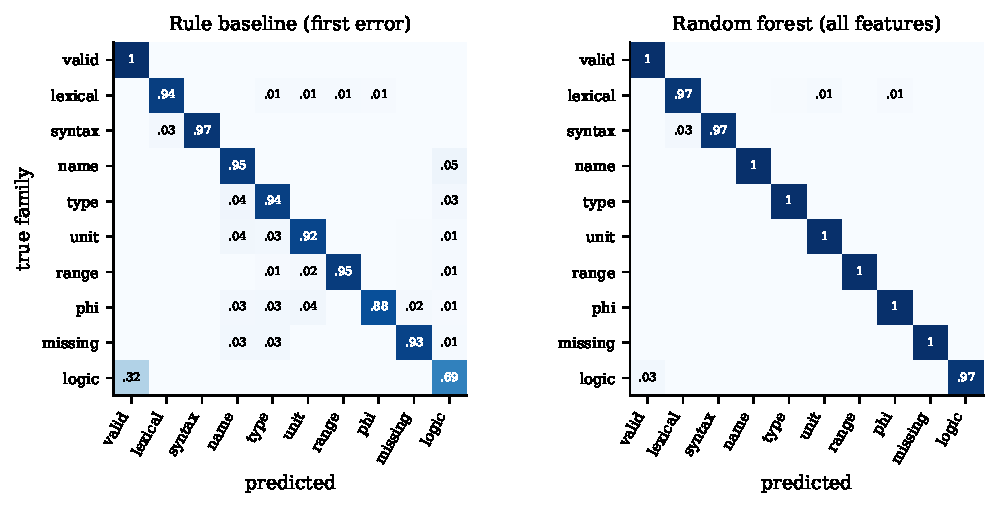
\includegraphics[width=\textwidth]{figs/confusion.pdf}
\caption{Row-normalised confusion matrices on the test set. Left: the ``first error'' rule. Right: random forest.}
\label{fig:confusion}
\end{figure*}

\begin{table}[t]
\centering
\caption{Per-class F1 of the rule baselines and precision, recall and F1 of the random forest.}
\label{tab:perclass}
\footnotesize
\adjustbox{max width=\columnwidth}{\begin{tabular}{lrrrrr}
\toprule
 & \multicolumn{2}{c}{\textbf{Rule F1}} & \multicolumn{3}{c}{\textbf{Random forest}}\\
\cmidrule(lr){2-3}\cmidrule(lr){4-6}
\textbf{Family} & first & severe & P & R & F1\\
\midrule
valid & 0.864 & 0.864 & 0.971 & 1.000 & 0.985\\
lexical & 0.959 & 0.777 & 0.975 & 0.970 & 0.972\\
syntax & 0.987 & 0.846 & 1.000 & 0.975 & 0.987\\
name & 0.913 & 1.000 & 1.000 & 1.000 & 1.000\\
type & 0.912 & 1.000 & 0.995 & 1.000 & 0.998\\
unit & 0.922 & 1.000 & 0.985 & 1.000 & 0.993\\
range & 0.967 & 1.000 & 1.000 & 1.000 & 1.000\\
phi & 0.931 & 1.000 & 0.990 & 1.000 & 0.995\\
missing & 0.946 & 1.000 & 1.000 & 1.000 & 1.000\\
logic & 0.755 & 0.813 & 1.000 & 0.970 & 0.985\\\bottomrule
\end{tabular}}
\end{table}

\begin{enumerate}
    \item \textbf{Faults the compiler cannot see.} 63 of the 200 test programs in the \emph{logic} class (31.5\%) are
    reported as clean by both rules, so their \emph{logic} recall is only \RuleLogicRecall\%. These are the inverted
    clinical rules and the mismatched alert texts: the programs are well formed, well typed and unit-correct. The random
    forest recovers them (\RFLogicRecall\% recall for \emph{logic}) using the pattern features, which count relational
    operators that point the wrong way relative to the alert vocabulary nearby. Six \emph{logic} programs are still
    taken for \emph{valid}.
    \item \textbf{Cascades hide the root cause of lexical faults.} The ``most severe family'' rule is perfect on all six
    semantic families, which is unsurprising because it implements the labelling rule. It fails on \emph{lexical}
    programs: an unterminated string swallows the rest of its line, the parser then reports follow-on syntax errors, and
    the priority rule, which ranks syntax above lexical, picks the symptom (73 of 200 programs). The ``first error''
    rule gets these right more often because the lexical error is reported first, but it pays for that elsewhere.
    \item \textbf{The first diagnostic is not always the root cause.} With two faults in the program, the ``first error''
    rule is correct on only \RuleFirstDouble\% of them, against 96.2\% on single-fault programs; the random forest is correct on
    \RFDouble\% of the two-fault programs.
    \item \textbf{What remains.} The forest makes 17 errors on 2{,}000 programs: six \emph{logic} programs taken for
    \emph{valid} (the soft faults above), five \emph{syntax} programs taken for \emph{lexical}, and six \emph{lexical}
    programs assigned to a semantic family (one \emph{type}, three \emph{unit}, two \emph{phi}). The lexical--syntax
    confusion is the same cascade ambiguity as before and is not fully resolved.
\end{enumerate}

None of this says that machine learning is better than a well-designed rule set \emph{for the faults the rules were
written for}: on those, a precise analyser is already at 100\%. The gain is concentrated in the cases that a
rule-based analyser misses or mislabels. It is also worth being clear about what the 99\% figure means. The test programs
come from the same generator as the training programs, so the learned model is evaluated on an in-distribution
sample; Section~\ref{sec:threats} discusses what that does and does not show.

\paragraph{What the forest relies on.} Table~\ref{tab:topfeat} lists the most important features. The most important one by a
wide margin is \code{worst\_family\_rank}, the compiler-derived rank of the most severe diagnostic family; the next ones are
counts of individual diagnostic codes. In other words, the learned classifier is largely a learned post-processor of the
compiler's output---which is what the architecture intends.

\begin{table}[t]
\centering
\caption{Top-eight random-forest feature importances (mean decrease in impurity).}
\label{tab:topfeat}
\footnotesize
\adjustbox{max width=\columnwidth}{\begin{tabular}{lr}
\toprule
\textbf{Feature} & \textbf{Importance}\\
\midrule
\texttt{worst\_family\_rank} & 0.142\\
\texttt{diag\_DOM002} & 0.053\\
\texttt{diag\_DOM001} & 0.051\\
\texttt{first\_phase\_sem} & 0.048\\
\texttt{diag\_SEM005} & 0.044\\
\texttt{first\_fam\_type} & 0.043\\
\texttt{diag\_DOM003} & 0.043\\
\texttt{first\_fam\_name} & 0.039\\\bottomrule
\end{tabular}}
\end{table}

\subsection{Which Feature Groups Matter, and How Much Data Is Needed (E2)}

Fig.~\ref{fig:learning} and Table~\ref{tab:learning} show test macro-F1 of a random forest trained on four feature
views with an increasing number of training programs per class (mean over five random draws).

\begin{figure}[t]
\centering
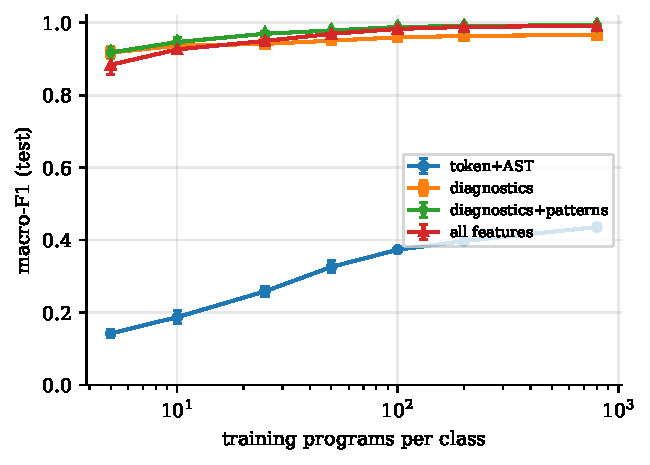
\includegraphics[width=\columnwidth]{figs/learning.pdf}
\caption{Learning curves of the random forest for four feature views (mean $\pm$ standard deviation over five draws).}
\label{fig:learning}
\end{figure}

\begin{table*}[t]
\centering
\caption{Test macro-F1 by feature view and number of training programs per class.}
\label{tab:learning}
\footnotesize
\adjustbox{max width=\textwidth}{\begin{tabular}{lrrrrrrr}
\toprule
\textbf{Feature view} & \textbf{5} & \textbf{10} & \textbf{25} & \textbf{50} & \textbf{100} & \textbf{200} & \textbf{800}\\
\midrule
token+AST & 0.142 & 0.187 & 0.258 & 0.326 & 0.373 & 0.398 & 0.436\\
diagnostics & 0.918 & 0.937 & 0.942 & 0.950 & 0.960 & 0.963 & 0.967\\
diagnostics+patterns & 0.918 & 0.946 & 0.970 & 0.979 & 0.988 & 0.991 & 0.994\\
all features & 0.884 & 0.926 & 0.950 & 0.969 & 0.983 & 0.988 & 0.991\\\bottomrule
\end{tabular}}
\end{table*}

Three observations follow.

\begin{itemize}
    \item \textbf{Surface features are not enough.} Token and tree statistics alone give a macro-F1 of only 0.14 with five
    programs per class and 0.44 with 800. A forest cannot recover from raw counts what a unit checker or a taint analysis
    computes. This is the strongest argument in the data for putting a real compiler front end underneath the learner.
    \item \textbf{Diagnostics carry most of the signal; patterns add the rest.} The diagnostic features alone plateau at
    0.967: they cannot see the soft logic faults. Adding the six pattern features lifts the curve to 0.994 at 800 programs per
    class.
    \item \textbf{More features are not better at small sample sizes.} The ``all features'' view is slightly \emph{worse}
    than diagnostics$+$patterns at every size (0.884 versus 0.918 at five programs per class, 0.991 versus 0.994 at 800). The
    token and tree features add 55 noisy dimensions that carry little information. We nevertheless kept the full 101-dimensional
    vector for the experiments with the GAN, because it is the representation the deployed classifier uses; a leaner view would be
    a reasonable simplification.
\end{itemize}

The scarce-data end of the curve is where it matters for the next experiment: with five labelled programs per class a forest
reaches a macro-F1 of 0.88, and the question is whether synthetic records can close part of the gap to 0.99.


% ============================================================
% RESULTS (part B): GAN augmentation and GAN anomaly detection
% ============================================================
\subsection{Augmentation under Scarcity: Does the GAN Help? (E3)}\label{sec:aug}

This experiment asks the question that motivated the use of a GAN: if only a handful of real faulty programs are available
per class, do synthetic feature vectors improve the classifier? Fig.~\ref{fig:augment} and
Tables~\ref{tab:augrf}--\ref{tab:augmlp} give the test macro-F1 of the seven regimes, averaged over ten seeds. The
\emph{valid} class always has 400 real training programs.

\begin{figure*}[t]
\centering
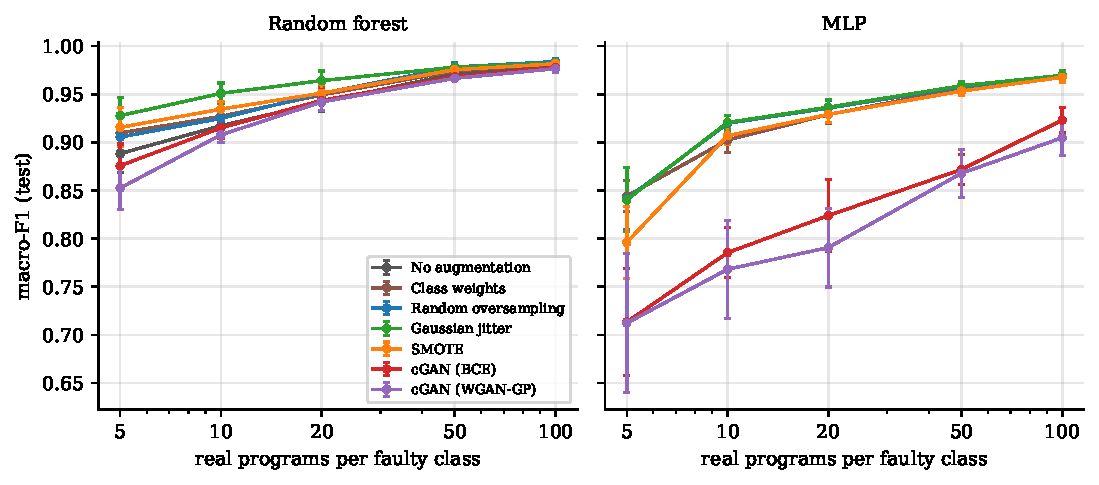
\includegraphics[width=\textwidth]{figs/augment.pdf}
\caption{Test macro-F1 against the number of real training programs per faulty class (mean $\pm$ standard deviation over ten
seeds). Left: random forest. Right: MLP.}
\label{fig:augment}
\end{figure*}

\begin{table*}[t]
\centering
\caption{Random forest: test macro-F1 (mean $\pm$ s.d., ten seeds) against the number of real programs per faulty class.
Bold marks the best mean in each column.}
\label{tab:augrf}
\footnotesize
\adjustbox{max width=\textwidth}{\begin{tabular}{lccccc}
\toprule
\textbf{Method} & \textbf{5} & \textbf{10} & \textbf{20} & \textbf{50} & \textbf{100}\\
\midrule
No augmentation & 0.888\,$\pm$\,0.020 & 0.917\,$\pm$\,0.009 & 0.942\,$\pm$\,0.009 & 0.971\,$\pm$\,0.003 & 0.979\,$\pm$\,0.003\\
Class weights & 0.910\,$\pm$\,0.018 & 0.927\,$\pm$\,0.008 & 0.949\,$\pm$\,0.008 & 0.974\,$\pm$\,0.004 & 0.982\,$\pm$\,0.003\\
Random oversampling & 0.906\,$\pm$\,0.020 & 0.925\,$\pm$\,0.010 & 0.951\,$\pm$\,0.009 & \textbf{0.978\,$\pm$\,0.004} & \textbf{0.984\,$\pm$\,0.003}\\
Gaussian jitter & \textbf{0.928\,$\pm$\,0.019} & \textbf{0.951\,$\pm$\,0.011} & \textbf{0.964\,$\pm$\,0.010} & 0.978\,$\pm$\,0.002 & 0.982\,$\pm$\,0.003\\
SMOTE & 0.916\,$\pm$\,0.020 & 0.935\,$\pm$\,0.008 & 0.951\,$\pm$\,0.009 & 0.975\,$\pm$\,0.005 & 0.982\,$\pm$\,0.003\\
cGAN (BCE) & 0.876\,$\pm$\,0.023 & 0.915\,$\pm$\,0.011 & 0.944\,$\pm$\,0.011 & 0.968\,$\pm$\,0.003 & 0.978\,$\pm$\,0.003\\
cGAN (WGAN-GP) & 0.853\,$\pm$\,0.022 & 0.908\,$\pm$\,0.008 & 0.942\,$\pm$\,0.009 & 0.967\,$\pm$\,0.001 & 0.977\,$\pm$\,0.004\\\bottomrule
\end{tabular}}
\end{table*}

\begin{table*}[t]
\centering
\caption{MLP: same protocol as Table~\ref{tab:augrf}.}
\label{tab:augmlp}
\footnotesize
\adjustbox{max width=\textwidth}{\begin{tabular}{lccccc}
\toprule
\textbf{Method} & \textbf{5} & \textbf{10} & \textbf{20} & \textbf{50} & \textbf{100}\\
\midrule
No augmentation & \textbf{0.844\,$\pm$\,0.016} & 0.902\,$\pm$\,0.013 & 0.929\,$\pm$\,0.009 & 0.956\,$\pm$\,0.005 & 0.969\,$\pm$\,0.004\\
Class weights & \textbf{0.844\,$\pm$\,0.016} & 0.902\,$\pm$\,0.013 & 0.929\,$\pm$\,0.009 & 0.956\,$\pm$\,0.005 & 0.969\,$\pm$\,0.004\\
Random oversampling & 0.842\,$\pm$\,0.032 & 0.920\,$\pm$\,0.008 & 0.936\,$\pm$\,0.008 & 0.958\,$\pm$\,0.005 & \textbf{0.970\,$\pm$\,0.005}\\
Gaussian jitter & 0.840\,$\pm$\,0.033 & \textbf{0.921\,$\pm$\,0.007} & \textbf{0.936\,$\pm$\,0.008} & \textbf{0.959\,$\pm$\,0.004} & 0.970\,$\pm$\,0.005\\
SMOTE & 0.796\,$\pm$\,0.038 & 0.907\,$\pm$\,0.010 & 0.929\,$\pm$\,0.008 & 0.953\,$\pm$\,0.005 & 0.968\,$\pm$\,0.005\\
cGAN (BCE) & 0.713\,$\pm$\,0.055 & 0.785\,$\pm$\,0.026 & 0.824\,$\pm$\,0.038 & 0.872\,$\pm$\,0.016 & 0.923\,$\pm$\,0.013\\
cGAN (WGAN-GP) & 0.712\,$\pm$\,0.073 & 0.768\,$\pm$\,0.051 & 0.791\,$\pm$\,0.041 & 0.868\,$\pm$\,0.025 & 0.905\,$\pm$\,0.018\\\bottomrule
\end{tabular}}
\end{table*}

\paragraph{The short answer is no.} With the random forest, the conditional GAN is never the best method and is usually
within noise of using no augmentation at all: at 20 real programs per class the BCE version scores 0.944 against 0.942 without
augmentation, and at 5 programs it is \emph{worse} (0.876 and 0.853 for the BCE and WGAN-GP versions, against 0.888). The
cheap alternatives help more. Gaussian jitter is the best method at every size up to 20 programs per class (0.928 against
0.888 at five programs), and SMOTE, random oversampling and class weights also give small gains. By 100 programs per class
all methods are within one point of each other. For the MLP the picture is worse for the GAN: its synthetic vectors cost
between 5 and 13 points of macro-F1 relative to no augmentation, with the largest damage at the smallest sizes
(0.713 against 0.844 at five programs per class), presumably because the MLP, unlike a forest, tries to fit every synthetic point.

Table~\ref{tab:augtests} gives paired comparisons over the ten seeds. The difference between the GAN and \emph{no augmentation}
is small and, depending on the size, indistinguishable from zero or slightly negative; the difference from jitter and SMOTE is
negative at every size. The $p$-values are uncorrected for the 30 comparisons shown, so they should be read as a rough guide.

\begin{table*}[t]
\centering
\caption{Paired difference in macro-F1 (random forest) between each GAN and three alternatives, with the two-sided
paired $t$-test $p$-value in parentheses. Negative values mean the GAN is worse.}
\label{tab:augtests}
\footnotesize
\adjustbox{max width=\textwidth}{\begin{tabular}{rlccc}
\toprule
\textbf{Real/class} & \textbf{GAN} & \textbf{vs.\ none} & \textbf{vs.\ SMOTE} & \textbf{vs.\ jitter}\\
\midrule
5 & cGAN (BCE) & -0.013 (0.034) & -0.040 (0.001) & -0.052 (0.001)\\
5 & cGAN (WGAN-GP) & -0.036 (0.007) & -0.063 (0.000) & -0.075 (0.000)\\
10 & cGAN (BCE) & -0.002 (0.163) & -0.019 (0.004) & -0.036 (0.000)\\
10 & cGAN (WGAN-GP) & -0.010 (0.016) & -0.027 (0.000) & -0.043 (0.000)\\
20 & cGAN (BCE) & +0.002 (0.378) & -0.008 (0.013) & -0.021 (0.000)\\
20 & cGAN (WGAN-GP) & +0.000 (0.920) & -0.009 (0.000) & -0.022 (0.000)\\
50 & cGAN (BCE) & -0.003 (0.010) & -0.008 (0.000) & -0.010 (0.000)\\
50 & cGAN (WGAN-GP) & -0.005 (0.001) & -0.009 (0.000) & -0.012 (0.000)\\
100 & cGAN (BCE) & -0.001 (0.015) & -0.004 (0.000) & -0.004 (0.000)\\
100 & cGAN (WGAN-GP) & -0.003 (0.002) & -0.005 (0.000) & -0.006 (0.000)\\\bottomrule
\end{tabular}}
\end{table*}

\paragraph{Where the benefit of augmentation lies.} Fig.~\ref{fig:augclass} breaks the result down by class for 20 real
programs per class. Most classes are already close to their ceiling without help. The exception is \emph{logic}, the family whose
members are partly invisible to the compiler and have to be recognised from the six pattern features: with five real programs
its F1 is 0.52 without augmentation, 0.79 with jitter, 0.70 with SMOTE and 0.47 with the BCE GAN; at 20 programs the values are
0.82, 0.93, 0.86 and 0.85. Augmentation in this setting is mostly a regulariser for the one hard class. The valid class
gains as a side effect, because fewer logic programs are mistaken for it.

\begin{figure*}[t]
\centering
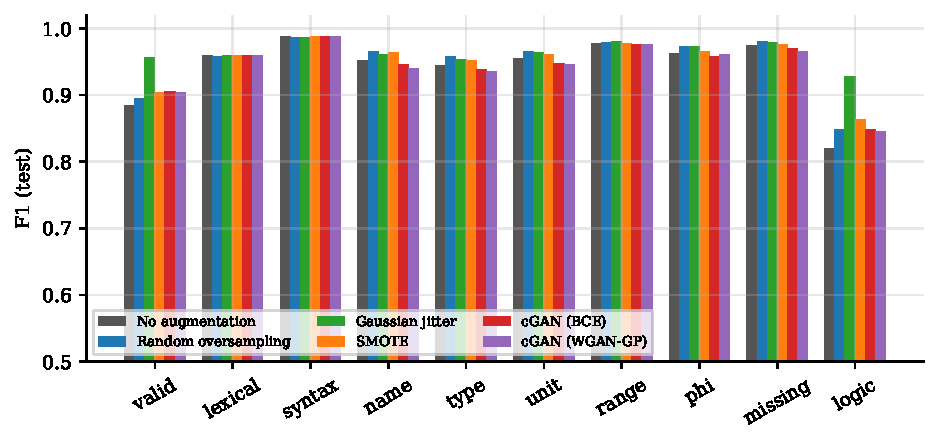
\includegraphics[width=\textwidth]{figs/augment_perclass.pdf}
\caption{Per-class F1 of the random forest with 20 real programs per faulty class (mean of ten seeds).}
\label{fig:augclass}
\end{figure*}

\paragraph{Why the GAN fails: fidelity of the synthetic vectors.} For one seed at 20 programs per class we checked
the synthetic vectors directly (Table~\ref{tab:fidelity}). \emph{Label validity} is the fraction of synthetic vectors that an
oracle random forest, trained on the full 8{,}000-program pool, assigns to the class the generator was asked for. \emph{NN distance}
is the mean standardised distance to the nearest real training vector of that class; for reference, held-out \emph{real}
programs of the same classes lie at a mean distance of \HeldoutNN{} from their nearest training example.

\begin{table}[t]
\centering
\caption{Fidelity of synthetic vectors (seed 0, 20 real programs per faulty class). Label validity for the three resampling methods is
high by construction: their points lie on or next to real training vectors that the oracle has itself seen.}
\label{tab:fidelity}
\footnotesize
\adjustbox{max width=\columnwidth}{\begin{tabular}{lrrr}
\toprule
\textbf{Generator} & \textbf{Label validity} & \textbf{NN distance} & \textbf{Exact copies (\%)}\\
\midrule
Random oversampling & 1.000 & 0.00 & 100.0\\
Gaussian jitter & 1.000 & 0.84 & 0.0\\
SMOTE & 1.000 & 3.01 & 0.0\\
cGAN (BCE) & 0.037 & 11.30 & 0.0\\
cGAN (WGAN-GP) & 0.043 & 10.80 & 0.0\\\bottomrule
\end{tabular}}
\end{table}

The result is stark. Only 4\% of the GAN's vectors are recognised as belonging to the requested class, which is below the
10\% expected from a classifier guessing among ten classes; the GAN vectors are also \emph{further} from the training data than genuinely
new real programs are. In other words, the generator has not learned the class-conditional structure. Fig.~\ref{fig:pca} shows the same thing
in two dimensions: the synthetic points (crosses) spread over the whole cloud of all classes instead of concentrating where the real
examples of the requested class lie, although a two-dimensional projection of mostly discrete count features is only a rough picture.

\begin{figure*}[t]
\centering
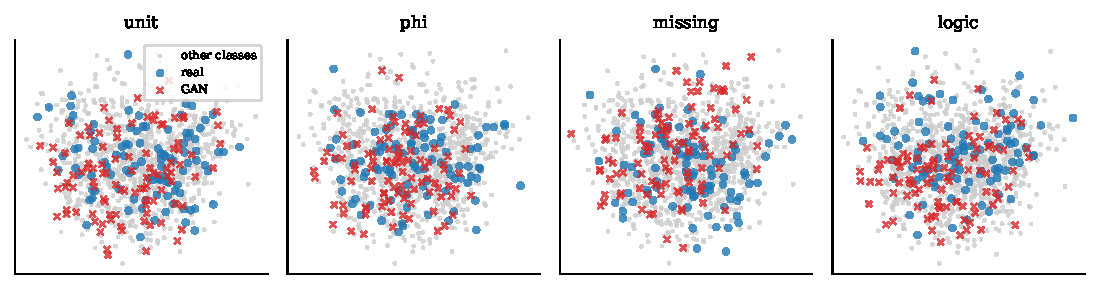
\includegraphics[width=\textwidth]{figs/gan_pca.pdf}
\caption{PCA projection of real (circles) and GAN-generated (crosses) vectors for four classes, with all other real vectors in grey
(a GAN trained on 100 real programs per class).}
\label{fig:pca}
\end{figure*}

We examined one likely cause. In the experiment above, mini-batches were drawn uniformly from the training set, which is dominated by the
400 \emph{valid} programs, so each rare class contributed only a few percent of the batches and the generator may have learned to ignore its
class input. We repeated the experiment (five seeds, 20 real programs per class) with class-balanced mini-batches, in which a class is chosen
first and an example second. Table~\ref{tab:gandiag} shows the outcome: label validity rises from roughly 4\% to 11--13\%, which is
about chance level, and macro-F1 does not improve. The imbalance in the batches therefore explains part of the failure but not the
rest. The remaining explanation is the one the numbers suggest: with 20 examples per class in a 101-dimensional space of counts,
a small unregularised GAN has too little to learn from, and a continuous generator blurs features that carry discrete, tightly coupled
meaning (for example, a diagnostic count of one for exactly one code). This follows the pattern commonly reported for GANs trained on very small tabular data, and it is a
limit of our setup rather than a general statement about GANs. We did not test architectures designed for tabular data, such as CTGAN
\cite{xu2019}, or any hyper-parameter search.

\begin{table}[t]
\centering
\caption{Effect of class-balanced mini-batches on the GAN (20 real programs per faulty class; mean $\pm$ s.d. over five seeds).
Label validity of about 0.10 is chance level.}
\label{tab:gandiag}
\footnotesize
\adjustbox{max width=\columnwidth}{\begin{tabular}{llcc}
\toprule
\textbf{Model} & \textbf{Mini-batches} & \textbf{Label validity} & \textbf{Macro-F1}\\
\midrule
cGAN (BCE) & uniform & 0.039\,$\pm$\,0.023 & 0.944\,$\pm$\,0.011\\
cGAN (WGAN-GP) & uniform & 0.045\,$\pm$\,0.005 & 0.944\,$\pm$\,0.008\\
cGAN (BCE) & class-balanced & 0.110\,$\pm$\,0.011 & 0.943\,$\pm$\,0.009\\
cGAN (WGAN-GP) & class-balanced & 0.126\,$\pm$\,0.009 & 0.935\,$\pm$\,0.010\\\bottomrule
\end{tabular}}
\end{table}

\paragraph{What the GAN is and is not good for here.} One property is worth noting: none of the synthetic vectors is an exact copy of a
real one (0\% exact copies in Table~\ref{tab:fidelity}), whereas random oversampling copies by definition. If privacy were the
goal, that would matter; but a synthetic set that does not carry the class signal is no use as training data either. Our
evidence supports a narrow conclusion: \emph{in this setting, with these model sizes and this amount of data, simple resampling
is the better way to handle rare error classes.}

\subsection{GAN-Based Anomaly Detection (E4)}

The second use of a GAN is to detect faulty programs when no faulty examples are available at all. A GAN is trained on the 800 valid
training programs; the negated discriminator output is the anomaly score. Table~\ref{tab:anomaly} and Fig.~\ref{fig:anomaly}
give the AUROC of each detector separating the 200 valid test programs from the 200 programs of each faulty family.

\begin{figure*}[t]
\centering
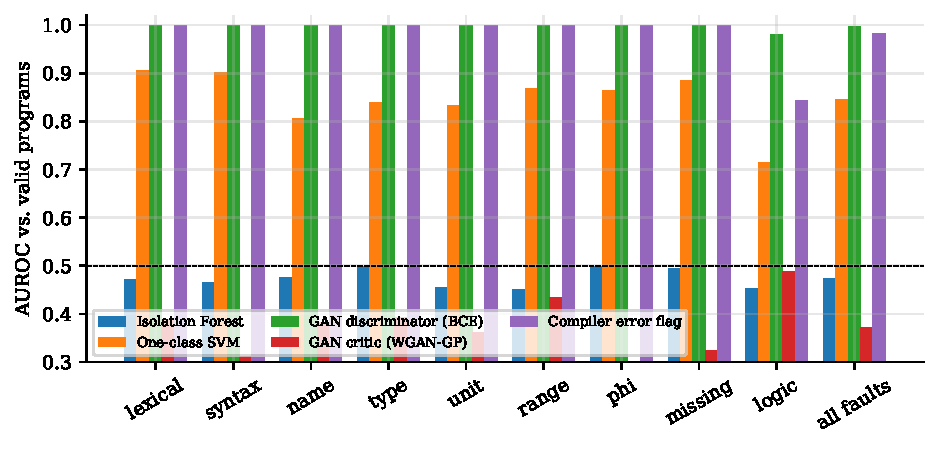
\includegraphics[width=\textwidth]{figs/anomaly.pdf}
\caption{AUROC of five detectors for valid versus faulty programs, by fault family (dashed line: chance).}
\label{fig:anomaly}
\end{figure*}

\begin{table*}[t]
\centering
\caption{AUROC of valid-versus-faulty detection by fault family. All detectors except the compiler flag were trained on
valid programs only.}
\label{tab:anomaly}
\footnotesize
\adjustbox{max width=\textwidth}{\begin{tabular}{lrrrrr}
\toprule
\textbf{Fault family} & \textbf{Isolation Forest} & \textbf{One-class SVM} & \textbf{GAN discriminator (BCE)} & \textbf{GAN critic (WGAN-GP)} & \textbf{Compiler error flag}\\
\midrule
lexical & 0.471 & 0.905 & 1.000 & 0.388 & 1.000\\
syntax & 0.465 & 0.901 & 1.000 & 0.310 & 1.000\\
name & 0.475 & 0.806 & 1.000 & 0.381 & 1.000\\
type & 0.498 & 0.839 & 1.000 & 0.392 & 1.000\\
unit & 0.454 & 0.834 & 1.000 & 0.360 & 1.000\\
range & 0.451 & 0.867 & 1.000 & 0.433 & 1.000\\
phi & 0.498 & 0.865 & 1.000 & 0.265 & 1.000\\
missing & 0.495 & 0.885 & 1.000 & 0.325 & 1.000\\
logic & 0.452 & 0.715 & 0.981 & 0.487 & 0.843\\
all faults & 0.473 & 0.846 & 0.998 & 0.371 & 0.982\\\bottomrule
\end{tabular}}
\end{table*}

The numbers need careful reading, because the headline is easy to over-interpret.

\begin{itemize}
    \item \textbf{The BCE discriminator is an excellent detector, but most of that is easy.} It reaches an AUROC of 0.998 over all faults. However,
    49 of the 101 features, including \emph{all} 40 diagnostic features, are constant on valid programs: a valid program reports no diagnostic. Any
    model that looks at those features can therefore tell a program with an error from one without. The compiler's own ``at least one error'' flag
    achieves 1.000 on every family except \emph{logic}, and it is a far simpler detector.
    \item \textbf{The informative column is \emph{logic}.} There the compiler flag falls to 0.843 (the soft faults raise no diagnostic), the one-class
    SVM reaches 0.715, and the BCE discriminator 0.981. To check that this is not a lucky seed, we retrained the discriminator with five seeds
    (Table~\ref{tab:anomalycheck}): the logic AUROC is 0.97--0.99 each time. It depends, however, on the pattern features: without them it drops to
    0.83--0.87, and the pattern features alone give only 0.60--0.69. So the discriminator's advantage comes from combining the
    compiler-derived signals with the pattern signal that valid programs never exhibit, and the pattern features were written with this fault in mind.
    \item \textbf{Isolation Forest is at chance (0.47).} We first suspected that it ignores the diagnostic features because they have zero range on the
    training data, so a random split cannot use them. Removing the constant features altogether changes nothing (0.473 to 0.475), which is consistent with that
    explanation: among the features that do vary, faulty programs look like valid ones.
    \item \textbf{The WGAN-GP critic fails.} Its AUROC is 0.37, \emph{below} chance: faulty programs receive a higher critic value than valid ones. A critic is
    trained to separate real from generated samples, not to model density, and outside the data it extrapolates. Negating the score would give about 0.63, but we report the
    score as defined in advance, not a sign chosen after seeing the result.
\end{itemize}

\begin{table}[t]
\centering
\caption{Stability and ablation of the BCE discriminator as anomaly detector (five seeds, mean $\pm$ s.d.).}
\label{tab:anomalycheck}
\footnotesize
\adjustbox{max width=\columnwidth}{\begin{tabular}{lcc}
\toprule
\textbf{Discriminator input} & \textbf{AUROC, logic} & \textbf{AUROC, all faults}\\
\midrule
All 101 features & 0.978\,$\pm$\,0.008 & 0.996\,$\pm$\,0.003\\
Without pattern features & 0.844\,$\pm$\,0.015 & 0.982\,$\pm$\,0.001\\
Pattern features only & 0.620\,$\pm$\,0.034 & 0.521\,$\pm$\,0.025\\\bottomrule
\end{tabular}}
\end{table}

The practical reading is modest. A GAN discriminator trained only on valid programs is a usable \emph{unsupervised} detector of the one family that the compiler
misses, but it is not better than the compiler on the families the compiler handles, and its result is only as good as the features it sees.

% ============================================================
% RESULTS (part C): compiler performance, case studies, validity
% ============================================================
\subsection{Compiler Performance and Optimisation (E5)}

\paragraph{Scaling.} Table~\ref{tab:scaling} and Fig.~\ref{fig:scaling} show the median compilation time for valid
programs of 46 to 12{,}016 lines (up to 88{,}000 tokens). A linear fit of total time against program size gives
\MsPerKloc{} ms per thousand lines ($R^2=\ScaleRSq$), so a 40-line program---the size of the corpus programs---compiles in
a few milliseconds. The log--log slope over the larger sizes is \ScaleSlope, i.e., growth is slightly worse than linear, and the
table shows where: the semantic phase, which takes roughly a quarter of the time for programs up to about 800 lines, accounts for more
than half of the total (53\%) at 12{,}000 lines. The reason is a known inefficiency of our implementation: every \code{if} copies the flow state
(the sets of assigned variables and facts), which grows with the number of top-level declarations, so a long flat program
pays a cost proportional to its size at every branch. Sharing the sets structurally between branches would remove this; at
the sizes of real clinical scripts it does not matter.

\begin{figure}[t]
\centering
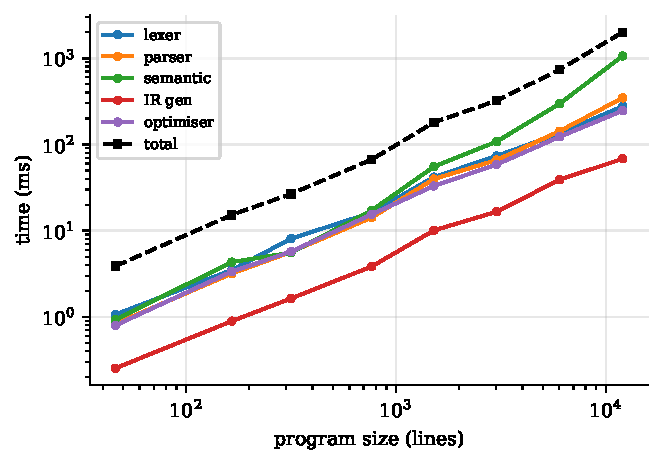
\includegraphics[width=\columnwidth]{figs/scaling.pdf}
\caption{Median compilation time per phase against program size (log--log).}
\label{fig:scaling}
\end{figure}

\begin{table*}[t]
\centering
\caption{Median time per phase in milliseconds, and IR size before and after optimisation.}
\label{tab:scaling}
\footnotesize
\adjustbox{max width=\textwidth}{\begin{tabular}{rrrrrrrrrr}
\toprule
\textbf{Lines} & \textbf{Tokens} & \textbf{Lex} & \textbf{Parse} & \textbf{Sem} & \textbf{IR} & \textbf{Opt} & \textbf{Total} & \textbf{IR ins.} & \textbf{Opt.\ ins.}\\
\midrule
46 & 323 & 1.1 & 0.8 & 0.9 & 0.3 & 0.8 & 3.9 & 84 & 73\\
165 & 1{,}201 & 3.5 & 3.2 & 4.3 & 0.9 & 3.4 & 15.3 & 389 & 338\\
316 & 2{,}303 & 8.1 & 5.7 & 5.6 & 1.6 & 5.7 & 26.7 & 774 & 673\\
766 & 5{,}603 & 16.2 & 14.2 & 17.2 & 3.8 & 15.4 & 66.9 & 1{,}924 & 1{,}673\\
1{,}515 & 11{,}101 & 41.8 & 39.7 & 55.3 & 10.1 & 33.0 & 179.8 & 3{,}839 & 3{,}338\\
3{,}016 & 22{,}103 & 73.4 & 65.9 & 107.8 & 16.6 & 58.5 & 322.1 & 7{,}674 & 6{,}673\\
6{,}015 & 44{,}101 & 134.6 & 142.4 & 296.6 & 39.0 & 122.5 & 735.0 & 15{,}339 & 13{,}338\\
12{,}016 & 88{,}103 & 276.4 & 346.4 & 1060.4 & 68.1 & 246.0 & 1997.4 & 30{,}674 & 26{,}673\\\bottomrule
\end{tabular}}
\end{table*}

\paragraph{Optimisation.} Over 300 generated valid programs the optimiser removed on average \OptMean\% of the
three-address instructions (maximum \OptMax\%). On every one of them, running the original and the optimised code on ten
random inputs produced identical output events (\OptMismatch{} mismatches in \OptPrograms{} programs). The generated programs
are written the way a person would write them and contain little redundancy, so the gain is modest. Programs with constant
arithmetic show more. For the program in Listing~\ref{lst:fold}, the optimiser folds the two constants, shares the repeated
product \code{per\_kg * weight}, and deletes the dead branch, reducing 18 instructions to 11 (39\%).

\begin{lstlisting}[language={},numbers=none,caption={Three-address code of \texttt{examples/fold\_demo.med} before (left column of rows) and after optimisation.},label={lst:fold}]
 before                            |  after
 t1 = 2 * 400.0                    |  LIMIT = 800.0
 LIMIT = t1                        |  margin@1 = 750.0
 t2 = LIMIT - 50.0                 |  t3 = 12.0 * weight
 margin@1 = t2                     |  a@3 = t3
 per_kg@2 = 12.0                   |  b@4 = t3          (CSE)
 t3 = per_kg@2 * weight            |  goto L1           (dead branch)
 a@3 = t3                          |  L1:
 t4 = per_kg@2 * weight            |  t7 = a@3 + b@4
 b@4 = t4                          |  t8 = t7 + margin@1
 t5 = 1 > 2                        |  param t8
 ifFalse t5 goto L1                |  t9 = call print, 1
 param 'never printed'             |
 t6 = call print, 1                |
 L1:                               |
 t7 = a@3 + b@4                    |
 t8 = t7 + margin@1                |
 param t8                          |
 t9 = call print, 1                |
\end{lstlisting}

The listing also shows two limits of the optimiser. A jump to the immediately following label is left behind (no peephole
pass), and propagation stops at labels, so \code{margin@1} is not substituted into \code{t8}. Both are
straightforward extensions and neither affects correctness.

\subsection{Worked Examples}

The command-line tool prints the compiler's diagnostics and, below them, the classifier's estimate of the root-cause family.
Listing~\ref{lst:phi} shows a program with four independent faults: PHI concatenated into output, a temperature
threshold with the decimal point dropped (reported twice, once by the range-of-input check and once by the plausibility check), and
a dose added to a weight. The classifier ranks \emph{phi} first, in agreement with the root-cause priority.

\begin{lstlisting}[language={},numbers=none,caption={Output of \texttt{medcheck.py examples/phi\_leak.med}.},label={lst:phi}]
== examples/phi_leak.med: 100 tokens, 4 error(s), 0 warning(s)
  12:19: error DOM002: protected health information reaches print() without anonymize()
      | print("patient: " + patient_name);
  13:10: error DOM001: comparison against 380, outside the declared range [30, 43] of 'temp'
      | if (temp > 380 degC) {
  13:12: error DOM001: value 380 degC is outside the plausible range [20.0, 45.0] degC
      | if (temp > 380 degC) {
  16:12: error SEM005: unit mismatch: [mg] + [kg]
      | print(dose + weight);
== learned root-cause estimate: phi 0.80, range 0.11, lexical 0.06
\end{lstlisting}

Listing~\ref{lst:syn} shows recovery from two syntax faults. The missing semicolon is reported at the end of the line
where it belongs, not at the \code{if} that exposed it, and parsing continues, so the missing parenthesis on the next line is also
found. Because syntax errors were reported, the semantic phase did not run.

\begin{lstlisting}[language={},numbers=none,caption={Output of \texttt{medcheck.py examples/syntax\_errors.med}.},label={lst:syn}]
== examples/syntax_errors.med: 44 tokens, 2 error(s), 0 warning(s)
  5:25: error SYN001: expected ';' but found 'if'
      | let fever = temp > 38.0 degC
  6:23: error SYN001: expected ')' but found '{'
      | if (fever && hr > 100 bpm {
== learned root-cause estimate: syntax 0.99, lexical 0.01, valid 0.00
\end{lstlisting}

The most interesting case is the one in which the compiler has nothing to say. In the file
\texttt{examples/\allowbreak inverted\_\allowbreak rule.med} the fever rule reads \code{if (temp < 38.0 degC)} and prints an alert called \emph{fever}. It compiles without a single
diagnostic. The tool then adds the line produced by the classifier, shown in Listing~\ref{lst:inv}: the forest assigns the program
to \emph{logic} with probability 0.77 and flags that the rule-based front end found nothing. This is a probability estimate from
a model trained on synthetic faults, not a proof, and the tool says so by wording it as a suspicion.

\begin{lstlisting}[language={},numbers=none,caption={Output of \texttt{medcheck.py examples/inverted\_rule.med}.},label={lst:inv}]
== examples/inverted_rule.med: 50 tokens, 0 error(s), 0 warning(s)
== learned root-cause estimate: logic 0.77, valid 0.20, name 0.02
   note: the rule-based front end found no error, but the classifier suspects a 'logic'
         fault (possible clinical-logic error)
\end{lstlisting}

\subsection{Threats to Validity and Limitations}\label{sec:threats}

We want to be explicit about what these results do and do not establish.

\begin{itemize}
    \item \textbf{Synthetic corpus, in-distribution test.} Training and test programs come from the same generator, built from
    the same sixteen blocks and mutated by the same operators. The near-perfect accuracy therefore measures how well the
    classifier has learned \emph{this} generator's faults. It says little about hand-written MedScript programs, and nothing at all
    about real clinical code in other languages. A study on real faulty scripts would be the real test.
    \item \textbf{The labels are defined by the injection.} A program's label is whatever fault we injected (with a documented priority
    for two faults). We checked that each fault manifests in the compiler, but not that a human reviewer would call it the root
    cause.
    \item \textbf{The strong rule baseline shares the labelling rule.} The ``most severe family'' rule is, by construction, the
    labelling rule applied to diagnostics. Its 100\% accuracy on the semantic families is therefore partly circular; its failures
    (cascading lexical faults, invisible logic faults) are the informative part.
    \item \textbf{The soft-fault detector uses a hand-written vocabulary.} The pattern features rely on a list of alert words. A
    program that names its alerts differently would defeat them. The classifier learns a statistical regularity of the generated
    programs, not clinical knowledge.
    \item \textbf{Scope of the experiment grid.} The range of scarcity levels in the GAN experiment was widened after a preliminary run on a
    separate, smaller corpus (different random seed), in which the GAN showed no advantage at five to twenty examples per class.
    Hyper-parameters of all methods were fixed beforehand and not tuned on the test set; they were also not tuned at all, so a
    better-tuned GAN could do better than reported.
    \item \textbf{Language and tooling.} MedScript is a small DSL, implemented in Python for clarity rather than speed.
\end{itemize}


\subsection{Summary of Findings}

\begin{enumerate}
    \item A purpose-built front end with clinical semantics detects, with 100\% recall, the faults it was designed for, and the learned classifier
    adds value mainly where the rules are blind (soft logic faults) or ambiguous (cascades, multiple faults): \RuleFirstAcc\% and \RulePrioAcc\% for the two rule baselines against
    \RFAcc\% for the forest.
    \item The information that matters is computed by the compiler. Token and tree statistics alone reach a macro-F1 of 0.44 with 800 programs per class.
    \item Conditional GANs trained on the feature vectors did \emph{not} improve classification with scarce data. Gaussian jitter and SMOTE were better, and
    the GAN's synthetic vectors were mostly not recognisable as the class they were meant to represent.
    \item A GAN discriminator trained on valid programs detects soft logic faults well (AUROC about 0.98), but its performance on other families is
    trivially explained by the diagnostic features, and the WGAN-GP critic was unusable for this purpose.
    \item The compiler is fast enough for interactive use (\MsPerKloc{} ms per thousand lines) and its optimiser preserved behaviour on all tested programs.
\end{enumerate}


% ============================================================
% CONCLUSION
% ============================================================
\section{Conclusion and Future Work}\label{sec:concl}

\subsection{Conclusion}

We set out to build an intelligent compiler for medical data-processing programs: a front end that understands the
constraints of the domain, plus a learned component that classifies errors and uses a GAN to cope with scarce labelled
data. The first two parts worked as intended; the third did not.

The compiler for MedScript implements the usual phases---scanner, recursive-descent parser with insertion and panic-mode recovery,
semantic analyser, three-address code, optimiser---and extends the semantic phase with checks that matter in healthcare:
unit-of-measure checking by dimension vectors, physiological plausibility by interval reasoning, taint tracking of protected
health information, flow-sensitive handling of optional values, definite assignment, and division-by-zero detection. All of the
38 unit tests pass, and on 300 generated programs the optimiser preserved observable behaviour on random inputs in every case. Compilation
time grows roughly linearly with program size at about \MsPerKloc{} ms per thousand lines.

For classification, a random forest over 101 compiler-derived features reached \RFAcc\% accuracy on 2{,}000 held-out programs, against
\RuleFirstAcc\% and \RulePrioAcc\% for two rule-based baselines. The gain comes from two situations that rules handle poorly: faults that
produce no diagnostic (inverted clinical rules), and programs in which cascades or several faults make the first diagnostic
misleading. The learning curves show that surface features of the source text are nearly useless on their own (macro-F1 0.44), so
the value of the learner depends on the compiler beneath it.

The GAN result is negative, and we think it is more useful reported than hidden. With 5 to 100 real programs per faulty class, conditional
GANs (BCE and WGAN-GP) gave no improvement over no augmentation for a random forest and a clear loss for an MLP, while Gaussian
jitter and SMOTE gave gains of up to four points of macro-F1. A direct check of the synthetic vectors explains why: they were recognised as the requested class
only about 4\% of the time, and class-balanced training batches raised that only to chance level. A GAN discriminator trained on valid programs did
turn out to be a good unsupervised detector of the faults the compiler misses (AUROC about 0.98), but that is a narrower use than the one the project began with.

\textbf{Limitations.} The corpus is generated, and the test programs come from the same generator as the training programs, so the accuracy figures describe the
generator's faults rather than the faults of real clinical code. The pattern features rely on a hand-written vocabulary. MedScript is a small DSL, not a language
that clinical programmers use today. The optimiser is deliberately simple. These limits are discussed in Section~\ref{sec:threats}.

\subsection{Future Work}

\begin{itemize}
    \item \textbf{Real data.} Evaluate on hand-written MedScript programs written by people who did not see the generator, and, more ambitiously, port the
    checks (units, PHI taint, optional values) to a mainstream clinical-scripting language such as Python or R through an AST-based analyser.
    \item \textbf{Better generative models.} Try tabular generators such as CTGAN with proper handling of discrete features, pretrain on the abundant
    valid class, and generate \emph{programs} rather than feature vectors, for instance by training a model over the mutation operators, so that synthetic examples can also be compiled and checked.
    \item \textbf{Learned localisation.} Predict not only the error family but the line at which a soft fault such as an inverted comparison occurs, for example with a
    graph neural network over the syntax tree.
    \item \textbf{Richer semantics.} Add implicit unit conversion with checked conversion factors, interval analysis through loops, inter-procedural taint with function
    summaries, and a three-valued treatment of missing values.
    \item \textbf{A stronger back end.} Global value numbering, propagation across basic blocks, and code generation to a real target such as LLVM IR, so that the pipeline is
    complete from source to machine code.
    \item \textbf{Human evaluation.} Study whether the root-cause estimate shortens the time a developer needs to find a fault compared with raw diagnostics.
\end{itemize}


% ============================================================
% APPENDICES
% ============================================================
\appendices
\section{MedScript Grammar}\label{app:grammar}

The grammar below is the one implemented by the recursive-descent parser. Terminals are in quotes; \code{ID},
\code{NUM}, \code{STR} and \code{UNIT} are token classes.

\begin{lstlisting}[language={}]
program    = { decl } ;
decl       = inputDecl | constDecl | funcDecl | stmt ;
inputDecl  = "input" ID ":" type [ "phi" ]
             [ "range" "(" signedNum "," signedNum ")" ] ";" ;
constDecl  = "const" ID ":" type "=" expr ";" ;
funcDecl   = "func" ID "(" [ param { "," param } ] ")" "->" type block ;
param      = ID ":" type ;
type       = ( "int" | "float" | "bool" | "string" | unitType ) [ "?" ] ;
unitType   = unitTerm { ( "*" | "/" ) unitTerm } ;
unitTerm   = UNIT [ "^" NUM ] ;

stmt       = letStmt | ifStmt | whileStmt | returnStmt | assignStmt
           | exprStmt | block ;
letStmt    = "let" ID [ ":" type ] [ "=" expr ] ";" ;
assignStmt = ID "=" expr ";" ;
ifStmt     = "if" "(" expr ")" block [ "else" ( ifStmt | block ) ] ;
whileStmt  = "while" "(" expr ")" block ;
returnStmt = "return" [ expr ] ";" ;
exprStmt   = expr ";" ;
block      = "{" { stmt } "}" ;

expr       = orExpr ;
orExpr     = andExpr { "||" andExpr } ;
andExpr    = eqExpr  { "&&" eqExpr } ;
eqExpr     = relExpr { ( "==" | "!=" ) relExpr } ;
relExpr    = addExpr { ( "<" | ">" | "<=" | ">=" ) addExpr } ;
addExpr    = mulExpr { ( "+" | "-" ) mulExpr } ;
mulExpr    = unary   { ( "*" | "/" | "%" ) unary } ;
unary      = ( "-" | "!" ) unary | primary ;
primary    = NUM [ unitType ] | STR | "true" | "false"
           | ID [ "(" [ expr { "," expr } ] ")" ] | "(" expr ")" ;
\end{lstlisting}

A unit suffix after a number extends over \code{/} only when the next token is a unit, so \code{15 mg/kg} is a single
literal while \code{15 mg / weight} is a division.

\section{Diagnostic Catalogue}\label{app:diag}
Table~\ref{tab:diagcat} lists the 23 diagnostic codes with their phase, severity and error family.


\begin{table*}[t]
\centering
\caption{Diagnostic codes of the MedScript compiler.}\label{tab:diagcat}
\scriptsize
\begin{tabular}{llllp{6.3cm}}
\toprule
\textbf{Code} & \textbf{Phase} & \textbf{Severity} & \textbf{Family} & \textbf{Meaning}\\
\midrule
LEX001 & lexer & error & lexical & illegal character\\
LEX002 & lexer & error & lexical & malformed number\\
LEX003 & lexer & error & lexical & unterminated string literal\\
SYN001 & parser & error & syntax & expected token not found\\
SYN002 & parser & error & syntax & unexpected token in expression\\
SYN003 & parser & error & syntax & unexpected end of file\\
SEM001 & semantic & error & name & undeclared identifier or function\\
SEM002 & semantic & error & name & redeclaration\\
SEM003 & semantic & error & name & use before initialisation\\
SEM009 & semantic & error & name & assignment to an input or constant\\
SEM004 & semantic & error & type & type mismatch\\
SEM006 & semantic & error & type & wrong argument count or type\\
SEM008 & semantic & error & type & condition is not boolean\\
SEM005 & semantic & error & unit & unit-of-measure mismatch\\
DOM001 & semantic & error & range & implausible value or threshold outside declared range\\
DOM002 & semantic & error & phi & PHI reaches an output sink\\
DOM003 & semantic & error & missing & optional value used without presence check\\
SEM007 & semantic & error & logic & missing return on some path\\
DOM004 & semantic & error & logic & division by constant zero\\
DOM005 & semantic & error & logic & divisor range includes zero\\
W001 & semantic & warning & logic & unreachable code\\
W002 & semantic & warning & valid & unused variable\\
W003 & semantic & warning & logic & constant condition\\
\bottomrule
\end{tabular}
\end{table*}

\section{Fault-Injection Operators}\label{app:ops}

Table~\ref{tab:ops} lists the operators together with the number of times each was attempted while building the
corpus and how often the resulting fault was kept. \emph{Tried} counts every attempt, including those where the
operator was not applicable to the sampled program (for example, removing an \code{anonymize} call from a program
that has none); \emph{Kept} counts attempts that produced a program in which the fault manifested. The percentage is
therefore a mixture of applicability and manifestation, and it is not a measure of compiler accuracy.

\begin{table*}[t]
\centering
\caption{Fault-injection operators and yield during corpus construction.}\label{tab:ops}
\scriptsize
\begin{tabular}{llp{5.2cm}rrr}
\toprule
\textbf{Family} & \textbf{Operator} & \textbf{Fault injected} & \textbf{Tried} & \textbf{Kept} & \textbf{\%}\\
\midrule
lexical & \texttt{lex\_illegal} & insert an illegal character & 332 & 332 & 100\\
 & \texttt{lex\_number} & malform a numeric literal & 311 & 307 & 99\\
 & \texttt{lex\_string} & drop a closing quote & 362 & 361 & 100\\
\midrule
syntax & \texttt{syn\_semicolon} & delete a semicolon & 170 & 170 & 100\\
 & \texttt{syn\_paren} & delete a closing parenthesis & 173 & 173 & 100\\
 & \texttt{syn\_close\_brace} & delete a closing brace & 175 & 175 & 100\\
 & \texttt{syn\_open\_brace} & delete an opening brace & 139 & 139 & 100\\
 & \texttt{syn\_operand} & delete a comparison operand & 167 & 167 & 100\\
 & \texttt{syn\_keyword} & misspell a keyword & 176 & 176 & 100\\
\midrule
name & \texttt{name\_typo} & misspell a variable use & 208 & 208 & 100\\
 & \texttt{name\_delete\_decl} & delete a declaration & 182 & 182 & 100\\
 & \texttt{name\_redecl} & duplicate a declaration & 156 & 151 & 97\\
 & \texttt{name\_uninit} & remove an initialiser & 185 & 142 & 77\\
 & \texttt{name\_func} & misspell a function call & 173 & 128 & 74\\
 & \texttt{name\_assign\_input} & assign to an input & 189 & 189 & 100\\
\midrule
type & \texttt{type\_string\_assign} & assign a string/bool to a number & 194 & 150 & 77\\
 & \texttt{type\_bool\_assign} & assign a number to a bool & 189 & 189 & 100\\
 & \texttt{type\_arity} & change an argument count & 202 & 148 & 73\\
 & \texttt{type\_cond} & use a number as a condition & 170 & 170 & 100\\
 & \texttt{type\_return} & return the wrong type & 210 & 162 & 77\\
 & \texttt{type\_float\_int} & assign a float to an int & 181 & 181 & 100\\
\midrule
unit & \texttt{unit\_swap\_literal} & swap the unit of a literal & 225 & 212 & 94\\
 & \texttt{unit\_drop} & drop the unit of a literal & 218 & 208 & 95\\
 & \texttt{unit\_decl} & change a declared input unit & 210 & 206 & 98\\
 & \texttt{unit\_rate} & pass a wrong dose-rate unit & 195 & 86 & 44\\
 & \texttt{unit\_return} & return a wrong unit & 231 & 74 & 32\\
 & \texttt{unit\_add} & add quantities of different units & 215 & 214 & 100\\
\midrule
range & \texttt{range\_literal} & implausible threshold literal & 295 & 267 & 91\\
 & \texttt{range\_threshold} & threshold outside declared range & 321 & 273 & 85\\
 & \texttt{range\_decl} & invert a declared range & 323 & 323 & 100\\
 & \texttt{range\_const} & implausible dose constant & 307 & 137 & 45\\
\midrule
phi & \texttt{phi\_direct} & print a PHI input & 202 & 202 & 100\\
 & \texttt{phi\_alias} & export an alias of PHI & 219 & 219 & 100\\
 & \texttt{phi\_concat} & concatenate PHI into output & 222 & 222 & 100\\
 & \texttt{phi\_removeanon} & remove an anonymize() call & 219 & 116 & 53\\
 & \texttt{phi\_func} & leak PHI through a function & 241 & 241 & 100\\
\midrule
missing & \texttt{miss\_unguard} & remove a presence guard & 442 & 192 & 43\\
 & \texttt{miss\_new\_use} & use an optional value unguarded & 402 & 402 & 100\\
 & \texttt{miss\_make\_optional} & make a required input optional & 410 & 406 & 99\\
\midrule
logic & \texttt{logic\_div\_zero} & divide by constant zero & 174 & 174 & 100\\
 & \texttt{logic\_range\_zero} & divisor range includes zero & 193 & 101 & 52\\
 & \texttt{logic\_missing\_return} & delete a return & 166 & 109 & 66\\
 & \texttt{logic\_unreachable} & code after return & 160 & 112 & 70\\
 & \texttt{logic\_inverted} & invert a clinical comparison & 154 & 148 & 96\\
 & \texttt{logic\_wrong\_message} & mismatch alert text and rule & 165 & 163 & 99\\
 & \texttt{logic\_constcond} & constant if-condition & 193 & 193 & 100\\
\bottomrule
\end{tabular}
\end{table*}

\section{Running the Code}\label{app:run}

The repository accompanying this paper has the following layout.

\begin{lstlisting}[language={}]
code/
  medscript/   lexer, parser, ast_nodes, semantic, ir, driver, equiv
               generator, mutations, corpus, features
  ml/          gan.py (conditional GAN), augment.py (SMOTE, jitter, ...)
  tests/       test_compiler.py (38 unit tests)
  examples/    triage_ok, phi_leak, inverted_rule, syntax_errors,
               missing_value, fold_demo (.med)
  medcheck.py  compiler + learned root-cause estimate
  run_experiments.py   make_figures.py
  results/     JSON results of every experiment
  models/      trained random-forest classifier
\end{lstlisting}

\begin{lstlisting}[language={}]
python -m unittest discover -s tests     # unit tests
python medcheck.py examples/phi_leak.med # compile + classify a program
python run_experiments.py                # all experiments (~45 min, 10 cores)
python make_figures.py                   # figures and LaTeX tables
\end{lstlisting}

\section*{Acknowledgment}
The authors thank Dr.\ Prakash Kumar Sarangi, School of Computer Science and Engineering (SCOPE), VIT-AP University, for guidance throughout the Compiler Design Lab.

% ============================================================
% REFERENCES
% ============================================================
\begin{thebibliography}{38}

\bibitem{aho2006}
A. V. Aho, M. S. Lam, R. Sethi, and J. D. Ullman,
\textit{Compilers: Principles, Techniques, and Tools},
2nd ed., Pearson/Addison-Wesley, 2006.

\bibitem{cooper2007}
K. D. Cooper and L. Torczon,
\textit{Engineering a Compiler},
2nd ed., Morgan Kaufmann, 2011.

\bibitem{appel1998}
A. W. Appel,
\textit{Modern Compiler Implementation in ML},
Cambridge University Press, 1998.

\bibitem{grune2008}
D. Grune and C. J. H. Jacobs,
\textit{Parsing Techniques: A Practical Guide},
2nd ed., Springer, 2008.

\bibitem{burke1987}
M. G. Burke and G. A. Fisher,
``A practical method for LR and LL syntactic error diagnosis and recovery,''
\textit{ACM Transactions on Programming Languages and Systems}, vol. 9, no. 2, pp. 164--197, 1987.

\bibitem{pierce2002}
B. C. Pierce,
\textit{Types and Programming Languages},
MIT Press, 2002.

\bibitem{nielson1999}
F. Nielson, H. R. Nielson, and C. Hankin,
\textit{Principles of Program Analysis},
Springer, 1999.

\bibitem{kennedy1994}
A. Kennedy,
``Dimension types,''
in \textit{Proc. European Symposium on Programming (ESOP)}, LNCS vol. 788, Springer, 1994, pp. 348--362.

\bibitem{enck2010}
W. Enck et al.,
``TaintDroid: An information-flow tracking system for realtime privacy monitoring on smartphones,''
in \textit{Proc. 9th USENIX Symposium on Operating Systems Design and Implementation (OSDI)}, 2010, pp. 393--407.

\bibitem{hipaa}
U.S. Department of Health and Human Services,
``Standards for privacy of individually identifiable health information,''
45 CFR Parts 160 and 164 (HIPAA Privacy Rule).

\bibitem{leveson1993}
N. G. Leveson and C. S. Turner,
``An investigation of the Therac-25 accidents,''
\textit{IEEE Computer}, vol. 26, no. 7, pp. 18--41, 1993.

\bibitem{mco1999}
Mars Climate Orbiter Mishap Investigation Board,
\textit{Phase I Report},
NASA, November 1999.

\bibitem{hindle2012}
A. Hindle, E. T. Barr, Z. Su, M. Gabel, and P. Devanbu,
``On the naturalness of software,''
in \textit{Proc. 34th International Conference on Software Engineering (ICSE)}, 2012, pp. 837--847.

\bibitem{allamanis2018}
M. Allamanis, E. T. Barr, P. Devanbu, and C. Sutton,
``A survey of machine learning for big code and naturalness,''
\textit{ACM Computing Surveys}, vol. 51, no. 4, article 81, 2018.

\bibitem{allamanis2018graphs}
M. Allamanis, M. Brockschmidt, and M. Khademi,
``Learning to represent programs with graphs,''
in \textit{Proc. International Conference on Learning Representations (ICLR)}, 2018.

\bibitem{gupta2017}
R. Gupta, S. Pal, A. Kanade, and S. Shevade,
``DeepFix: Fixing common C language errors by deep learning,''
in \textit{Proc. AAAI Conference on Artificial Intelligence}, 2017, pp. 1345--1351.

\bibitem{pradel2018}
M. Pradel and K. Sen,
``DeepBugs: A learning approach to name-based bug detection,''
\textit{Proc. ACM on Programming Languages}, vol. 2, no. OOPSLA, article 147, 2018.

\bibitem{goodfellow2014}
I. Goodfellow et al.,
``Generative adversarial nets,''
in \textit{Advances in Neural Information Processing Systems 27}, 2014.

\bibitem{mirza2014}
M. Mirza and S. Osindero,
``Conditional generative adversarial nets,''
arXiv:1411.1784, 2014.

\bibitem{salimans2016}
T. Salimans, I. Goodfellow, W. Zaremba, V. Cheung, A. Radford, and X. Chen,
``Improved techniques for training GANs,''
in \textit{Advances in Neural Information Processing Systems 29}, 2016.

\bibitem{arjovsky2017}
M. Arjovsky, S. Chintala, and L. Bottou,
``Wasserstein generative adversarial networks,''
in \textit{Proc. 34th International Conference on Machine Learning (ICML)}, PMLR vol. 70, 2017, pp. 214--223.

\bibitem{gulrajani2017}
I. Gulrajani, F. Ahmed, M. Arjovsky, V. Dumoulin, and A. Courville,
``Improved training of Wasserstein GANs,''
in \textit{Advances in Neural Information Processing Systems 30}, 2017.

\bibitem{choi2017}
E. Choi, S. Biswal, B. Malin, J. Duke, W. F. Stewart, and J. Sun,
``Generating multi-label discrete patient records using generative adversarial networks,''
in \textit{Proc. Machine Learning for Healthcare Conference (MLHC)}, PMLR vol. 68, 2017, pp. 286--305.

\bibitem{xu2019}
L. Xu, M. Skoularidou, A. Cuesta-Infante, and K. Veeramachaneni,
``Modeling tabular data using conditional GAN,''
in \textit{Advances in Neural Information Processing Systems 32}, 2019.

\bibitem{antoniou2017}
A. Antoniou, A. Storkey, and H. Edwards,
``Data augmentation generative adversarial networks,''
arXiv:1711.04340, 2017.

\bibitem{chawla2002}
N. V. Chawla, K. W. Bowyer, L. O. Hall, and W. P. Kegelmeyer,
``SMOTE: Synthetic minority over-sampling technique,''
\textit{Journal of Artificial Intelligence Research}, vol. 16, pp. 321--357, 2002.

\bibitem{he2009}
H. He and E. A. Garcia,
``Learning from imbalanced data,''
\textit{IEEE Transactions on Knowledge and Data Engineering}, vol. 21, no. 9, pp. 1263--1284, 2009.

\bibitem{schlegl2017}
T. Schlegl, P. Seeb\"ock, S. M. Waldstein, U. Schmidt-Erfurth, and G. Langs,
``Unsupervised anomaly detection with generative adversarial networks to guide marker discovery,''
in \textit{Proc. Information Processing in Medical Imaging (IPMI)}, LNCS vol. 10265, Springer, 2017, pp. 146--157.

\bibitem{liu2008}
F. T. Liu, K. M. Ting, and Z.-H. Zhou,
``Isolation forest,''
in \textit{Proc. IEEE International Conference on Data Mining (ICDM)}, 2008, pp. 413--422.

\bibitem{scholkopf2001}
B. Sch\"olkopf, J. C. Platt, J. Shawe-Taylor, A. J. Smola, and R. C. Williamson,
``Estimating the support of a high-dimensional distribution,''
\textit{Neural Computation}, vol. 13, no. 7, pp. 1443--1471, 2001.

\bibitem{breiman2001}
L. Breiman,
``Random forests,''
\textit{Machine Learning}, vol. 45, no. 1, pp. 5--32, 2001.

\bibitem{pedregosa2011}
F. Pedregosa et al.,
``Scikit-learn: Machine learning in Python,''
\textit{Journal of Machine Learning Research}, vol. 12, pp. 2825--2830, 2011.

\bibitem{paszke2019}
A. Paszke et al.,
``PyTorch: An imperative style, high-performance deep learning library,''
in \textit{Advances in Neural Information Processing Systems 32}, 2019.

\bibitem{kingma2015}
D. P. Kingma and J. Ba,
``Adam: A method for stochastic optimization,''
in \textit{Proc. International Conference on Learning Representations (ICLR)}, 2015.

\bibitem{sokolova2009}
M. Sokolova and G. Lapalme,
``A systematic analysis of performance measures for classification tasks,''
\textit{Information Processing \& Management}, vol. 45, no. 4, pp. 427--437, 2009.

\bibitem{fawcett2006}
T. Fawcett,
``An introduction to ROC analysis,''
\textit{Pattern Recognition Letters}, vol. 27, no. 8, pp. 861--874, 2006.

\bibitem{muchnick1997}
S. S. Muchnick,
\textit{Advanced Compiler Design and Implementation},
Morgan Kaufmann, 1997.

\bibitem{lattner2004}
C. Lattner and V. Adve,
``LLVM: A compilation framework for lifelong program analysis and transformation,''
in \textit{Proc. International Symposium on Code Generation and Optimization (CGO)}, 2004, pp. 75--88.

\end{thebibliography}



\end{document}
